\documentclass{beamer}

% xcolor and define colors -------------------------
\usepackage{xcolor}

% https://www.viget.com/articles/color-contrast/
\definecolor{purple}{HTML}{5601A4}
\definecolor{navy}{HTML}{0D3D56}
\definecolor{ruby}{HTML}{9a2515}
\definecolor{alice}{HTML}{107895}
\definecolor{daisy}{HTML}{EBC944}
\definecolor{coral}{HTML}{F26D21}
\definecolor{kelly}{HTML}{829356}
\definecolor{cranberry}{HTML}{E64173}
\definecolor{jet}{HTML}{131516}
\definecolor{asher}{HTML}{555F61}
\definecolor{slate}{HTML}{314F4F}

% Mixtape Sessions
\definecolor{picton-blue}{HTML}{00b7ff}
\definecolor{violet-red}{HTML}{ff3881}
\definecolor{sun}{HTML}{ffaf18}
\definecolor{electric-violet}{HTML}{871EFF}

% Main theme colors
\definecolor{accent}{HTML}{00b7ff}
\definecolor{accent2}{HTML}{871EFF}
\definecolor{gray100}{HTML}{f3f4f6}
\definecolor{gray800}{HTML}{1F292D}


% Beamer Options -------------------------------------

% Background
\setbeamercolor{background canvas}{bg = white}

% Change text margins
\setbeamersize{text margin left = 15pt, text margin right = 15pt} 

% \alert
\setbeamercolor{alerted text}{fg = accent2}

% Frame title
\setbeamercolor{frametitle}{bg = white, fg = jet}
\setbeamercolor{framesubtitle}{bg = white, fg = accent}
\setbeamerfont{framesubtitle}{size = \small, shape = \itshape}

% Block
\setbeamercolor{block title}{fg = white, bg = accent2}
\setbeamercolor{block body}{fg = gray800, bg = gray100}

% Title page
\setbeamercolor{title}{fg = gray800}
\setbeamercolor{subtitle}{fg = accent}

%% Custom \maketitle and \titlepage
\setbeamertemplate{title page}
{
    %\begin{centering}
        \vspace{20mm}
        {\Large \usebeamerfont{title}\usebeamercolor[fg]{title}\inserttitle}\\
        {\large \itshape \usebeamerfont{subtitle}\usebeamercolor[fg]{subtitle}\insertsubtitle}\\ \vspace{10mm}
        {\insertauthor}\\
        {\color{asher}\small{\insertdate}}\\
    %\end{centering}
}

% Table of Contents
\setbeamercolor{section in toc}{fg = accent!70!jet}
\setbeamercolor{subsection in toc}{fg = jet}

% Button 
\setbeamercolor{button}{bg = accent}

% Remove navigation symbols
\setbeamertemplate{navigation symbols}{}

% Table and Figure captions
\setbeamercolor{caption}{fg=jet!70!white}
\setbeamercolor{caption name}{fg=jet}
\setbeamerfont{caption name}{shape = \itshape}

% Bullet points

%% Fix left-margins
\settowidth{\leftmargini}{\usebeamertemplate{itemize item}}
\addtolength{\leftmargini}{\labelsep}

%% enumerate item color
\setbeamercolor{enumerate item}{fg = accent}
\setbeamerfont{enumerate item}{size = \small}
\setbeamertemplate{enumerate item}{\insertenumlabel.}

%% itemize
\setbeamercolor{itemize item}{fg = accent!70!white}
\setbeamerfont{itemize item}{size = \small}
\setbeamertemplate{itemize item}[circle]

%% right arrow for subitems
\setbeamercolor{itemize subitem}{fg = accent!60!white}
\setbeamerfont{itemize subitem}{size = \small}
\setbeamertemplate{itemize subitem}{$\rightarrow$}

\setbeamertemplate{itemize subsubitem}[square]
\setbeamercolor{itemize subsubitem}{fg = jet}
\setbeamerfont{itemize subsubitem}{size = \small}


% Special characters

\usepackage{collectbox}

\makeatletter
\newcommand{\mybox}{%
    \collectbox{%
        \setlength{\fboxsep}{1pt}%
        \fbox{\BOXCONTENT}%
    }%
}
\makeatother





% Links ----------------------------------------------

\usepackage{hyperref}
\hypersetup{
  colorlinks = true,
  linkcolor = accent2,
  filecolor = accent2,
  urlcolor = accent2,
  citecolor = accent2,
}


% Line spacing --------------------------------------
\usepackage{setspace}
\setstretch{1.1}


% \begin{columns} -----------------------------------
\usepackage{multicol}


% Fonts ---------------------------------------------
% Beamer Option to use custom fonts
\usefonttheme{professionalfonts}

% \usepackage[utopia, smallerops, varg]{newtxmath}
% \usepackage{utopia}
\usepackage[sfdefault,light]{roboto}

% Small adjustments to text kerning
\usepackage{microtype}



% Remove annoying over-full box warnings -----------
\vfuzz2pt 
\hfuzz2pt


% Table of Contents with Sections
\setbeamerfont{myTOC}{series=\bfseries, size=\Large}
\AtBeginSection[]{
        \frame{
            \frametitle{Roadmap}
            \tableofcontents[current]   
        }
    }


% Tables -------------------------------------------
% Tables too big
% \begin{adjustbox}{width = 1.2\textwidth, center}
\usepackage{adjustbox}
\usepackage{array}
\usepackage{threeparttable, booktabs, adjustbox}
    
% Fix \input with tables
% \input fails when \\ is at end of external .tex file
\makeatletter
\let\input\@@input
\makeatother

% Tables too narrow
% \begin{tabularx}{\linewidth}{cols}
% col-types: X - center, L - left, R -right
% Relative scale: >{\hsize=.8\hsize}X/L/R
\usepackage{tabularx}
\newcolumntype{L}{>{\raggedright\arraybackslash}X}
\newcolumntype{R}{>{\raggedleft\arraybackslash}X}
\newcolumntype{C}{>{\centering\arraybackslash}X}

% Figures

% \imageframe{img_name} -----------------------------
% from https://github.com/mattjetwell/cousteau
\newcommand{\imageframe}[1]{%
    \begin{frame}[plain]
        \begin{tikzpicture}[remember picture, overlay]
            \node[at = (current page.center), xshift = 0cm] (cover) {%
                \includegraphics[keepaspectratio, width=\paperwidth, height=\paperheight]{#1}
            };
        \end{tikzpicture}
    \end{frame}%
}

% subfigures
\usepackage{subfigure}


% Highlight slide -----------------------------------
% \begin{transitionframe} Text \end{transitionframe}
% from paulgp's beamer tips
\newenvironment{transitionframe}{
    \setbeamercolor{background canvas}{bg=accent!40!black}
    \begin{frame}\color{accent!10!white}\LARGE\centering
}{
    \end{frame}
}


% Table Highlighting --------------------------------
% Create top-left and bottom-right markets in tabular cells with a unique matching id and these commands will outline those cells
\usepackage[beamer,customcolors]{hf-tikz}
\usetikzlibrary{calc}
\usetikzlibrary{fit,shapes.misc}

% To set the hypothesis highlighting boxes red.
\newcommand\marktopleft[1]{%
    \tikz[overlay,remember picture] 
        \node (marker-#1-a) at (0,1.5ex) {};%
}
\newcommand\markbottomright[1]{%
    \tikz[overlay,remember picture] 
        \node (marker-#1-b) at (0,0) {};%
    \tikz[accent!80!jet, ultra thick, overlay, remember picture, inner sep=4pt]
        \node[draw, rectangle, fit=(marker-#1-a.center) (marker-#1-b.center)] {};%
}

\usepackage{breqn} % Breaks lines

\usepackage{amsmath}
\usepackage{mathtools}

\usepackage{pdfpages} % \includepdf

\usepackage{listings} % R code
\usepackage{verbatim} % verbatim

% Video stuff
\usepackage{media9}

% packages for bibs and cites
\usepackage{natbib}
\usepackage{har2nat}
\newcommand{\possessivecite}[1]{\citeauthor{#1}'s \citeyearpar{#1}}
\usepackage{breakcites}
\usepackage{alltt}

% Setup math operators
\DeclareMathOperator{\E}{E} \DeclareMathOperator{\tr}{tr} \DeclareMathOperator{\se}{se} \DeclareMathOperator{\I}{I} \DeclareMathOperator{\sign}{sign} \DeclareMathOperator{\supp}{supp} \DeclareMathOperator{\plim}{plim}
\DeclareMathOperator*{\dlim}{\mathnormal{d}\mkern2mu-lim}
\newcommand\independent{\protect\mathpalette{\protect\independenT}{\perp}}
   \def\independenT#1#2{\mathrel{\rlap{$#1#2$}\mkern2mu{#1#2}}}
\newcommand*\colvec[1]{\begin{pmatrix}#1\end{pmatrix}}

\newcommand{\myurlshort}[2]{\href{#1}{\textcolor{gray}{\textsf{#2}}}}


\begin{document}

\imageframe{./lecture_includes/mixtape_did_cover.png}



% ---- Content ----

\section{Introduction}

\subsection{Managing expectations}



\begin{frame}{Introductions}

\begin{itemize}
\item Thank you for welcoming me to Egham and Royal Holloway!
\item Scott Cunningham, Professor at Baylor, Waco Texas (halfway between Dallas and Austin) 
\item Welcome to a two day workshop on difference-in-differences and if we have time synthetic control!  
\end{itemize}

\end{frame}





\begin{frame}{What my pedagogy is like}

\begin{itemize}
\item Long days that don't feel long because it's high energy, with regular breaks including lunch
\item Move between the econometrics, history of thought, videos, applications, code, spreadsheets, exercises
\item Ask questions at any point; I'll do my best to answer them
\end{itemize}

\end{frame}


\begin{frame}{Class goals}
Pedagogical goal is to break down the procedures into plain English, rebuilding it into something you can and want to use, but also:

  \begin{enumerate}
    \item \textbf{Confidence}: You will feel like you have a good enough understanding of diff-in-diff and synthetic control, both in its basics and some more contemporary issues, so that by the end of the week it a very intuitive, friendly, and useful tool
    \item \textbf{Comprehension}: You will have learned a lot both conceptually and in the specifics, particularly with regards to issues around identification and estimation in the diff-in-diff and synth context
    \item \textbf{Competency}: You will have more knowledge of programming syntax in Stata and R so that later you can apply this in your own work
  \end{enumerate}

\end{frame}



\begin{frame}{Day 1 outline}

Introduction to DiD basics 
	\begin{itemize}
	\item Potential outcomes review and the ATT parameter
	\item DiD equation (``four averages and three differences''), parallel trends and estimation with OLS
	\item Evaluating parallel trends with falsifications, event studies 
	\item Compositional changes, triple differences and covariates
	\end{itemize}

\end{frame}


\begin{frame}{Day 2 outline}

 Differential timing
	\begin{itemize}
	\item TWFE Pathologies in static and dynamic specifications (``event study'')
	\item Aggregating group-time ATT
	\end{itemize}

\bigskip

Synthetic control (non-negative and negative weighting)	

\end{frame}



\subsection{Diff-in-diff background}


\begin{frame}{What is difference-in-differences (DiD)}

\begin{itemize}
\item DiD is a very old, relatively straightforward, intuitive research design
\item A group of units are assigned some treatment and then compared to a group of units that weren't
\item One of the most widely used quasi-experimental methods in economics and increasingly in industry
\item Mostly associated with ``big shocks'' happening in space over time
\end{itemize}


\begin{quote}
``A good way to do econometrics is to look for good natural experiments and use statistical methods that can tidy up the confounding factors that nature has not controlled for us.'' -- Daniel McFadden (Nobel Laureate recipient with Heckman 2002)
\end{quote}

\end{frame}


\begin{frame}

	\begin{figure}
	\caption{Currie, et al. (2020)}
	\includegraphics[scale=0.25]{./lecture_includes/currie_did.png}
	\end{figure}


\end{frame}




\begin{frame}{Origins of diff-in-diff}

\begin{itemize}
\item Difference-in-differences (DiD) was quietly and largely unnoticed introduced in the 19th century as a way to convince skeptics in health policy arguments
\item Dominant disease theory in 19th century was \emph{miasma} -- disease caused by smelly vapor
\item Keep in mind -- microorganisms would not be identified until much later, partly caused by poor resolution in microscopes (Freedman 2007)

\end{itemize}

\end{frame}

\begin{frame}{Miasma I: Ignaz Semmelweis and washing hands}

\begin{itemize}
\item 1840s, Vienna maternity wards had high postpartum infections in one wing compared to other wings
\item One division had doctors and trainee doctors, but another had midwives and trainee midwives
\end{itemize}

\end{frame}

\begin{frame}{Miasma I: Ignaz Semmelweis and washing hands}

\begin{itemize}
\item Ignaz Semmelweis notes the difference in 1841 when hospitals moved to ``anatomical'' training involving cadavers (Pamela Jakeila lecture notes on DiD)
\item New training happens to one but not the other and Semmelweis thinks the mortality is caused by working with cadavers
\item Proposes washing hands with chlorine in 1847 in the midwives' wing and uses a DiD design of pre and post
\end{itemize}

\end{frame}



\begin{frame}{Miasma II: John Snow and cholera}

\begin{itemize}
\item Three major waves of cholera in the early to mid 1800s in London
\item John Snow believed cholera was spread through the Thames water supply which contradicted dominant theory about ``dirty air'' transmission
\item Grand experiment: Lambeth moves its pipe between 1849 and 1854; Southwark and Vauxhall delay
\item He can evaluate the effect in three ways (one of which is DiD)
\end{itemize}

\end{frame}


\begin{frame}

	\begin{figure}
	\caption{Two water utility companies in London 1854}
	\includegraphics[scale=0.225]{./lecture_includes/lambeth.png}
	\end{figure}


\end{frame}




\begin{frame}{1) Simple cross-sectional design}

\begin{table}\centering
		\caption{Lambeth and Southwark and Vauxhall, 1854}
		\begin{center}
		\begin{tabular}{ll}
		\toprule
		\multicolumn{1}{l}{\textbf{Company}}&
		\multicolumn{1}{c}{\textbf{Cholera mortality}}\\
		\midrule
		Lambeth  & $Y=L + D$ \\
		Southwark and Vauxhall  & $Y=SV$ \\
		\bottomrule
		\end{tabular}
		\end{center}
	\end{table}

\bigskip

\begin{eqnarray*}
\widehat{\delta}_{cs} = D + (L-SV)
\end{eqnarray*}What is $L$ and $SV$?  

\end{frame}

\begin{frame}{1) Simple cross-sectional design}

\begin{table}\centering
		\caption{Lambeth and Southwark and Vauxhall, 1854}
		\begin{center}
		\begin{tabular}{ll}
		\toprule
		\multicolumn{1}{l}{\textbf{Company}}&
		\multicolumn{1}{c}{\textbf{Cholera mortality}}\\
		\midrule
		Lambeth  & $Y=L + D$ \\
		Southwark and Vauxhall  & $Y=SV$ \\
		\bottomrule
		\end{tabular}
		\end{center}
	\end{table}

\bigskip

\begin{eqnarray*}
\widehat{\delta}_{cs} = D + (L-SV)
\end{eqnarray*}This is biased if $\L \neq SV$ (selection bias). Give an example when we're pretty sure they are equal.

\end{frame}

\begin{frame}{2) Interrupted time series design}

	\begin{table}\centering
		\caption{Lambeth, 1849 and 1854}
		\begin{center}
		\begin{tabular}{lll}
		\toprule
		\multicolumn{1}{l}{\textbf{Company}}&
		\multicolumn{1}{c}{\textbf{Time}}&
		\multicolumn{1}{c}{\textbf{Cholera mortality}}\\
		\midrule
		Lambeth & 1849 & $Y=L$ \\
		& 1854 & $Y=L + (T + D)$ \\
		\bottomrule
		\end{tabular}
		\end{center}
	\end{table}

\begin{eqnarray*}
\widehat{\delta}_{its} = D + T
\end{eqnarray*}What is required for this estimator to be unbiased?


\end{frame}

\begin{frame}{3) Difference-in-differences}

\begin{table}\centering
		\caption{Lambeth and Southwark and Vauxhall, 1849 and 1854}
		\begin{center}
		\begin{tabular}{lll|lc}
		\toprule
		\multicolumn{1}{l}{\textbf{Companies}}&
		\multicolumn{1}{c}{\textbf{Time}}&
		\multicolumn{1}{c}{\textbf{Outcome}}&
		\multicolumn{1}{c}{$D_1$}&
		\multicolumn{1}{c}{$D_2$}\\
		\midrule
		Lambeth & Before & $Y=L$ \\
		& After & $Y=L + T_L + D$ & $T_L+D$\\
		\midrule
		& & & & $D$ \\
		\midrule
		Southwark and Vauxhall & Before & $Y=SV$ \\
		& After & $Y=SV + T_{SV}$ & $T_{SV}$\\
		\bottomrule
		\end{tabular}
		\end{center}
	\end{table}

\begin{eqnarray*}
\widehat{\delta}_{did} = D + (T_L - T_{SV})
\end{eqnarray*}This method yields an unbiased estimate of D if $T_{SV} = \textcolor{red}{T_L}$

\end{frame}


\begin{frame}{Orley goes to Washington}

\begin{itemize}
\item Orley Ashenfelter graduated from Princeton in the 1970s, takes a job in Washington DC and begins studying ``job trainings programs''
\item Empirical crisis in empirical macro and empirical labor back in the 1970s -- Orley, David Card, Bob Lalonde, Alan Krueger at Princeton all helped bring attention to it and began pushing for solutions, one of which was RCTs in labor but also diff-in-diff as well as better instruments
\item Listen to Orley explain the connection he made between twoway fixed effects and difference-in-differences; it was born out of a need to explain OLS to an American bureaucrat

\end{itemize}

\url{https://youtu.be/WnB3EJ8K7lg?t=126}

\end{frame}

\begin{frame}{Steps of a project}

\begin{enumerate}
\item Convert research question into causal parameter
\item Deduce beliefs needed to estimate that causal parameter with data
\item Create a calculator that will use data and estimate the causal parameter
\end{enumerate}

\bigskip

Most of us skip (1) and maybe even (2) and instead simply ``run regressions'' and cross our fingers that that coefficient is causal, but is it? And why is it?  And what is it?  Let's dig into Orley's comment a little more. 

\end{frame}

\subsection{Potential outcomes}

\begin{frame}{Equivalence}
$$Y_{ist} = \alpha_0 + \alpha_1 Treat_{is} + \alpha_2 Post_{t} + \textcolor{blue}{\delta} (Treat_{is} \times Post_t) + \varepsilon_{ist} $$

\bigskip

$$\widehat{\textcolor{blue}{\delta}} = \bigg ( \overline{y}_k^{post(k)} - \overline{y}_k^{pre(k)} \bigg ) - \bigg ( \overline{y}_U^{post(k)} - \overline{y}_U^{pre(k)} \bigg ) $$

\begin{itemize}
\item Orley claims that the OLS estimator of $\delta$ and the ``four averages and three subtractions'' are the same thing numerically
\item And they are -- they are numerically \emph{identical}
\item And under a particular assumption, they are also unbiased estimates of an aggregate causal parameter
\item But to see this we need new notation -- potential outcomes
\end{itemize}

\end{frame}





\begin{frame}{Potential outcomes notation}
	
	\begin{itemize}
	\item Let the treatment be a binary variable: $$D_{i,t} =\begin{cases} 1 \text{ if in job training program $t$} \\ 0 \text{ if not in job training program at time $t$} \end{cases}$$where $i$ indexes an individual observation, such as a person

	\end{itemize}
\end{frame}

\begin{frame}{Potential outcomes notation}
	
	\begin{itemize}

	\item Potential outcomes: $$Y_{i,t}^j =\begin{cases} 1 \text{: wages at time $t$ if trained} \\ 0 \text{: wages at time $t$ if not trained} \end{cases}$$where $j$ indexes a counterfactual state of the world

	\end{itemize}
\end{frame}



\begin{frame}{Treatment effect definitions}


	\begin{block}{Individual treatment effect}
	    The individual treatment effect,  $\delta_i$, equals $Y_i^1-Y_i^0$
	\end{block}

Missing data problem:  I don't know my own counterfactual
	
\end{frame}


\begin{frame}{Conditional Average Treatment Effects}	
	\begin{block}{Average Treatment Effect on the Treated (ATT)}
	The average treatment effect on the treatment group is equal to the average treatment effect conditional on being a treatment group member:
		\begin{eqnarray*}
		E[\delta|D=1]&=&E[Y^1-Y^0|D=1] \nonumber \\
		&=&E[Y^1|D=1]-\textcolor{red}{E[Y^0|D=1]}
		\end{eqnarray*}
	\end{block}
	
	\bigskip

This is one of the most important policy parameters, if not the most important, and coincidentally it's also the parameter you get with diff-in-diff (even with heterogeneity)

	
\end{frame}

\begin{frame}{Potential outcomes vs data}

\begin{itemize}
\item ATT is expressed in terms of potential outcomes, but we do not use potential outcomes for estimation; we use data
\item Potential outcomes are unknown and \emph{hypothetical} possibilities describing states of the world but our data are realized outcomes, or ``data'', that actually occurred
\item Potential outcomes become realized under treatment assignment $$Y_{it}=D_{it}Y_{it}^1 + (1-D_{it})Y_{it}^0$$
\item Depending on how the treatment is assigned really dictates whether correlations reveal causal effects or bias

\end{itemize}
\end{frame}

\subsection{Estimation}


\begin{frame}{DiD equation}

Orley's ``four averages and three subtractions'', or what Bacon will call the 2x2

\begin{eqnarray*}
\widehat{\delta} = \bigg ( E[Y_k|Post] - E[Y_k|Pre] \bigg ) - \bigg ( E[Y_U | Post ] - E[ Y_U | Pre] \bigg) \\
\end{eqnarray*}$k$ are the people in the job training program, $U$ are the untreated people not in the program, $Post$ is after the trainees took the class, $Pre$ is the period just before they took the class, and $E[y]$ is mean earnings. 

\bigskip

Does $\widehat{\delta}$ equal the ATT?  If so when? If not why not?

\end{frame}



\begin{frame}{Potential outcomes and the switching equation}

\begin{eqnarray*}
\widehat{\delta} &=& \bigg ( \underbrace{E[Y^1_k|Post] - E[Y^0_k|Pre] \bigg ) - \bigg ( E[Y^0_U | Post ] - E[ Y^0_U | Pre]}_{\mathclap{\text{Switching equation}}} \bigg)  \\
&&+ \underbrace{\textcolor{red}{E[Y_k^0 |Post] - E[Y^0_k | Post]}}_{\mathclap{\text{Adding zero}}} 
\end{eqnarray*}

\end{frame}

\begin{frame}{Parallel trends bias}

\begin{eqnarray*}
\widehat{\delta} &=& \underbrace{E[Y^1_k | Post] - \textcolor{red}{E[Y^0_k | Post]}}_{\mathclap{\text{ATT}}} \\
&& + \bigg [  \underbrace{\textcolor{red}{E[Y^0_k | Post]} - E[Y^0_k | Pre] \bigg ] - \bigg [ E[Y^0_U | Post] - E[Y_U^0 | Pre] }_{\mathclap{\text{Non-parallel trends bias in 2x2 case}}} \bigg ]
\end{eqnarray*}


\end{frame}

\begin{frame}{Identification through parallel trends}
	

	\begin{block}{Parallel trends}
	Assume two groups, treated and comparison group, then we define parallel trends as:	 $$\textcolor{red}{E(}\textcolor{red}{\Delta Y^0_k)} = E(\Delta Y^0_U)$$
	\end{block}

\textbf{In words}: ``The \textcolor{red}{evolution of earnings for our trainees \emph{had they not trained}} is the same as the evolution of mean earnings for non-trainees''.  

\bigskip

It's in \textcolor{red}{red} because parallel trends is untestable and critically important to estimation of the ATT using any method, OLS or ``four averages and three subtractions''

	

	
\end{frame}


\begin{frame}{What is parallel trends}

\begin{itemize}
\item Parallel trends assumes away the selection bias associated with comparisons
\item The assumption is thought to be more plausible than simply assuming simple comparisons held equal $E[Y^0|D=0]=E[Y^0|D=1]$
\item But it is still a strong assumption, and differs from the assumptions have in the RCT which though also untestable, is nearly guaranteed by randomization
\item Most of the hard part of the work involves the old fashioned detective work and the work of making good arguments with good exhibits (tables and figures)
\end{itemize}

\end{frame}



\begin{frame}{Understanding parallel trends through worksheets}

Before we move into regression, let's go through a simple exercise to really pin down these core ideas with simple calculations

\bigskip 

\url{https://docs.google.com/spreadsheets/d/1onabpc14JdrGo6NFv0zCWo-nuWDLLV2L1qNogDT9SBw/edit?usp=sharing}

\end{frame}



\begin{frame}{OLS Specification}
	
	\begin{itemize}
	\item Simple DiD equation will identify ATT under parallel trends
	\item But so will a particular OLS specification (two groups and no covariates)
	\item OLS was historically preferred because
		\begin{itemize}
		\item OLS estimates the ATT under parallel trends
		\item Easy to calculate the standard errors
		\item Easy to include multiple periods
		\end{itemize}
	\item People liked it also because of differential timing, continuous treatments and covariates, but those are more complex so we address them later
	\end{itemize}
\end{frame}

\begin{frame}{Minimum wages}

\begin{itemize}
\item Card and Krueger (1994) have a famous study estimating causal effect (ATT) of minimum wages on employment
\item Exploited a policy change in New Jersey between February and November in mid-1990s where minimum wage was increased, but neighbor PA did not
\item Using DiD, they do not find a negative effect of the minimum wage on employment which is part of its legacy today, but I mainly present it to illustrate the history and the design principles
\end{itemize}

\end{frame}

\begin{frame}
	\begin{figure}
	\includegraphics[scale=0.5]{./lecture_includes/minwage_whore}
	\end{figure}
\end{frame}

\begin{frame}{Card on that study}

\begin{quote}
``I’ve subsequently stayed away from the minimum wage literature for a number of reasons. First, it cost me a lot of friends. People that I had known for many years, for instance, some of the ones I met at my first job at the University of Chicago, became very angry or disappointed. They thought that in publishing our work we were being traitors to the cause of economics as a whole.''
\end{quote}

\bigskip

But let's listen to Orley's opinion about the paper's controversy at the time.  \url{https://youtu.be/MOtbuRX4eyQ?t=1882}

\end{frame}


\begin{frame}{OLS specification of the DiD equation}
	
	\begin{itemize}
	\item The correctly specified OLS regression is an interaction with time and group fixed effects:$$Y_{its} = \alpha + \gamma NJ_s + \lambda d_t + \delta (NJ \times d)_{st} + \varepsilon_{its}$$
		\begin{itemize}
		\item NJ is a dummy equal to 1 if the observation is from NJ
		\item d is a dummy equal to 1 if the observation is from November (the post period)
		\end{itemize}
	\item This equation takes the following values
		\begin{itemize}
		\item PA Pre: $\alpha$
		\item PA Post: $\alpha + \lambda$
		\item NJ Pre: $\alpha + \gamma$
		\item NJ Post: $\alpha + \gamma + \lambda + \delta$
		\end{itemize}
	\item DiD equation: (NJ Post - NJ Pre) - (PA Post - PA Pre) $= \delta$
	\end{itemize}
\end{frame}




\begin{frame}[plain]
	$$Y_{ist} = \alpha + \gamma NJ_s + \lambda d_t + \delta(NJ\times d)_{st} + \varepsilon_{ist}$$
	\begin{figure}
	\includegraphics[scale=0.90]{./lecture_includes/waldinger_dd_5.pdf}
	\end{figure}
\end{frame}


\begin{frame}[plain]
	$$Y_{ist} = \alpha + \gamma NJ_s + \lambda d_t + \delta(NJ\times d)_{st} + \varepsilon_{ist}$$
	\begin{figure}
	\includegraphics[scale=0.90]{./lecture_includes/waldinger_dd_5.pdf}
	\end{figure}

Notice how OLS is ``imputing'' $E[Y^0|D=1,Post]$ for the treatment group in the post period? It is only ``correct'', though, if parallel trends is a good approximation

\end{frame}


\begin{frame}{Inference}
	
	\begin{itemize}
	\item  Bertrand, Duflo and Mullainathan (2004) show that conventional standard errors will often severely understate the standard deviation of the estimators
	\item Standard errors are biased downward (i.e., too small, over reject)
	\item They proposed three solutions, but most only use one of them (clustering)
	\end{itemize}
\end{frame}


\begin{frame}{Inference}
	
		\begin{enumerate}
		\item[1 ] Block bootstrapping standard errors (if you analyze states the block should be the states and you would sample whole states with replacement for bootstrapping)
		\item[2 ] Clustering standard errors at the group level (in Stata one would simply add \texttt{, cluster(state)} to the regression equation if one analyzes state level variation)
		\end{enumerate}

\bigskip

Most people will simply cluster, but there are issues if you have too few clusters. They mention a third way but it's only a curiosity.
		
\end{frame}

\begin{frame}{Sample code}

Let's show that the ``four averages and three differences'' yields the same number as our saturated regression now using \texttt{equivalence.do} at github labs under ``Basic DID''

\end{frame}

\begin{frame}{Main DiD assumptions}

There are actually three DiD assumptions in the basic design, but you usually only hear about the first:

\bigskip

\begin{enumerate}
\item Parallel trends -- concerns changes in $Y^0$, one of which is a fictional change because the post treatment $Y^0$ doesn't exist for the treated
\item No anticipation (next slide)
\item SUTVA (slide after next)
\end{enumerate}

\end{frame}

\begin{frame}{No Anticipation}

\begin{itemize}
\item No anticipation means that the treatment effect happens only at the time that the treatment occurs or after, but not before
	\begin{itemize}
	\item \textbf{Example 1}: Tomorrow I win the lottery, but don't get paid yet. I decide to buy a new house today. That violates NA
	\item \textbf{Example 2}: Next year, a state lets you drive without a driver license and you know it. But you can't drive without a driver license today.  This satisfies NA.
	\end{itemize}
\item We need this for a boring reason -- baseline in the DiD \emph{must} be $Y^0$ in order for DiD to equal ATT plus PT 
\end{itemize}

\end{frame}

\begin{frame}{SUTVA}

\begin{itemize}
\item Stable Unit Treatment Value Assumption (Imbens and Rubin 2015) focuses on what happens when in our analysis we are combining units (versus defining treatment effects)
	\begin{enumerate}
	\item \textbf{No Interference}: a treated unit cannot impact a control unit such that their potential outcomes change (unstable treatment value)
	\item \textbf{No hidden variation in treatment}: When units are indexed to receive a treatment, their dose is the same as someone else with that same index
	\item \textbf{Scale}: If scaling causes interference or changes inputs in production process, then \#1 or \#2 are violated
	\end{enumerate}
\item Shifts from defining treatment effects to estimating them, which means being careful about who is the control group, how you define treatments and what questions can and cannot be answered with this method
\end{itemize}

\end{frame}



\section{Types of parallel trends evidence}

\subsection{How parallel trends can get violated}




\begin{frame}{Violating parallel trends exercise}

\begin{itemize}
\item Parallel trends are needed so we can impute the missing $E[Y^0|D=1]$ with $E[Y^0|D=0]$ either explicitly or implicitly
\item Which means if parallel trends isn't true, then the imputation isn't correct and therefore estimates are biased
\item To illustrate this, let's go through the document again -- this time to tab 2
\end{itemize}

\url{https://docs.google.com/spreadsheets/d/1onabpc14JdrGo6NFv0zCWo-nuWDLLV2L1qNogDT9SBw/edit?usp=sharing}

\end{frame}


\begin{frame}{Violating parallel trends}

\begin{itemize}
\item Parallel trends are in expectation only -- we don't rely everybody to follow the same trend, just that the group average for $Y^0$ be approximately the same for treated and control 
\item Violations are a form of selection bias and there are two straightforward ways that parallel trends will be violated
	\begin{enumerate}
	\item Compositional differences in samples associated with repeated cross-sections
	\item Policy endogeneity
	\end{enumerate}
\end{itemize}

\end{frame}



\begin{frame}{Repeated cross-sections and compositional change}
	
	\begin{itemize}
	\item One of the risks of a repeated cross-section is that the composition of the sample may have changed between the pre and post period in ways that are correlated with treatment
	\item Hong (2013) uses repeated cross-sectional data from the Consumer Expenditure Survey (CEX) containing music expenditure and internet use for a random sample of households
	\item Study exploits the emergence of Napster (first file sharing software widely used by Internet users) in June 1999 as a natural experiment
	\item Study compares internet users and internet non-users before and after emergence of Napster
	\end{itemize}

\end{frame}

\begin{frame}[plain]
	\begin{figure}
	\includegraphics{./lecture_includes/Hong_1.pdf}
	\end{figure}
	
\end{frame}

\begin{frame}[shrink=20,plain]
	\begin{figure}
	\includegraphics{./lecture_includes/Hong_2.pdf}
	\end{figure}
	
	Diffusion of the Internet changes samples (e.g., younger music fans are early adopters)
	
\end{frame}

\begin{frame}{Repeated cross-sections}

\begin{itemize}
\item Surprisingly underappreciated problem with almost no literature around it
\item So what can you do?  Check covariate balance by regressing the time-varying covariates instead of the outcome onto the treatment using your OLS specification
\item They should be exogenous remember, so this covariate regression can be a helpful test of whether this is a problem
\item ``Difference-in-differences with Compositional Changes'' by Pedro Sant'anna and Qi Xu (not yet released) is the only paper I've ever seen to look into it
\end{itemize}

\end{frame}


\subsection{Event studies}

\begin{frame}{Types of evidence}

What kinds of evidence is convincing?

\begin{itemize}
\item You are building a case, the prosecutor before a judge and jury, always in battle with the defense attorney
\item Evidence has particular broadly defined forms that can help you on the front end
\item Your goal in my humble opinion should be reasonable and theoretically relevant falsifications with particular kinds of data visualization, starting with the event study
\end{itemize}

\end{frame}


\begin{frame}{Event studies have become mandatory in DiD}

	\begin{figure}
	\includegraphics[scale=0.5]{./lecture_includes/currie_eventstudy.png}
	\end{figure}

\end{frame}

\begin{frame}{Event studies are about pre-trends not parallel trends}

\begin{itemize}
	\item Parallel trends involves, $Y^0$, specifically $\Delta E[\textcolor{red}{Y^0}|D=1] = \Delta E[Y^0|D=0]$ 
		\begin{itemize}
		\item  Notice that parallel trends is about $Y^0$ in other words, not $Y^1$
		\end{itemize}
	\item We cannot verify the \textcolor{red}{red} term, because the change is post-treatment and thus counterfactual (fictional)
	\item But there are other non-red $\Delta E[Y^0|D=1]$ that aren't fictional which we can investigate, but where?
\end{itemize}

\bigskip

``Pre-trends'' are also $\Delta E[Y^0|D=1]$, just non-fictional in nature

\bigskip

Testing for parallel pre-trends is a type of falsification for selection bias

\end{frame}

\begin{frame}{Intuition behind event studies}
	
	\begin{itemize}
	\item Checking pre-trends is \textbf{not} a test for parallel trends as there is no formal test for parallel trends
	\item It's akin to finding a smoking gun -- maybe someone planted it, but dismiss it is irresponsible
	\item Do not overweight nor underweight parallel pre-trends
	\item Even if pre-trends are the same one still has to worry about other policies changing at the same time (omitted variable bias is a parallel trends violation)

\end{itemize}

\end{frame}


\begin{frame}{How do we do it?}

\begin{itemize}
\item Formula is ``four averages and three differences'' on each lead and lag relative to baseline so calculate it using OLS or manually
\item Some prefer to also plotting raw data
\end{itemize}

\end{frame}

\begin{frame}{Plot the raw data when there's only two groups}

	\begin{figure}
	\includegraphics[scale=2.5]{./lecture_includes/waldinger_dd_6.pdf}
	\end{figure}

\end{frame}




\begin{frame}{Event study regression}
	
	\begin{itemize}
	\item Event studies have a simple OLS specification with only one treatment group and one never-treated group $$Y_{its} = \alpha +  \sum_{\tau=-2}^{-q}\mu_{\tau}D_{s\tau} + \sum_{\tau=0}^m\delta_{\tau}D_{s\tau}+\varepsilon_{ist}$$
		\begin{itemize}
		\item where $D$ is an interaction of the treatment dummy with the calendar year 
		\item Treatment occurs in year 0, no anticipation, drop baseline $t-1$
		\item All ``four averages and three differences'' calculations will use $t-1$ as ``pre'' which is why it must be untreated (no anticipation)
		\item Includes $q$ leads or anticipatory effects and $m$ lags or post treatment effects
		\end{itemize}
	\end{itemize}
\end{frame}

\begin{frame}{Event study regression}


$$Y_{its} = \alpha + \sum_{\tau=-2}^{-q}\mu_{\tau}D_{s\tau} + \sum_{\tau=0}^m\delta_{\tau}D_{s\tau}+\varepsilon_{ist}$$

\bigskip

Typically you'll plot the coefficients and 95\% CI on all leads and lags (binned or not, trimmed or not) 

\bigskip

Under no anticipation, then you expect $\widehat{\mu}$ coefficients to be zero, which gives you confidence that parallel trends holds (but is not a guarantee, and there are still specification issues -- see Jon Roth's work)

\bigskip

Under parallel trends, $\widehat{\delta}$ are estimates of the ATT at points in time

\end{frame}



\begin{frame}{Medicaid and Affordable Care Act example}

\begin{figure}
\includegraphics[scale=0.25]{./lecture_includes/medicaid_qje}
\end{figure}

\end{frame}

\begin{frame}{Types of evidence}

\begin{itemize}
\item \textbf{Bite} -- show that the expansion shifted people into Medicaid and out of uninsured status
\item \textbf{Main Results} -- Show your main results (the point of the paper)
\item \textcolor{red}{\textbf{Placebos}} -- Show that there's no effect on mortality for groups it shouldn't be affecting (people 65+)
\item \textcolor{blue}{\textbf{Mechanisms}} -- Find some reason explaining why the treatment affects the outcome via some ``mechanism''
\item \textbf{Event study} -- Show leads and lags on mortality
\end{itemize}

\end{frame}


\imageframe{./lecture_includes/Miller_Medicaid1.png}

\imageframe{./lecture_includes/Miller_Medicaid2.png}

\imageframe{./lecture_includes/Miller_Medicaid3.png}


\begin{frame}{Falsifications on elderly}

	\begin{figure}
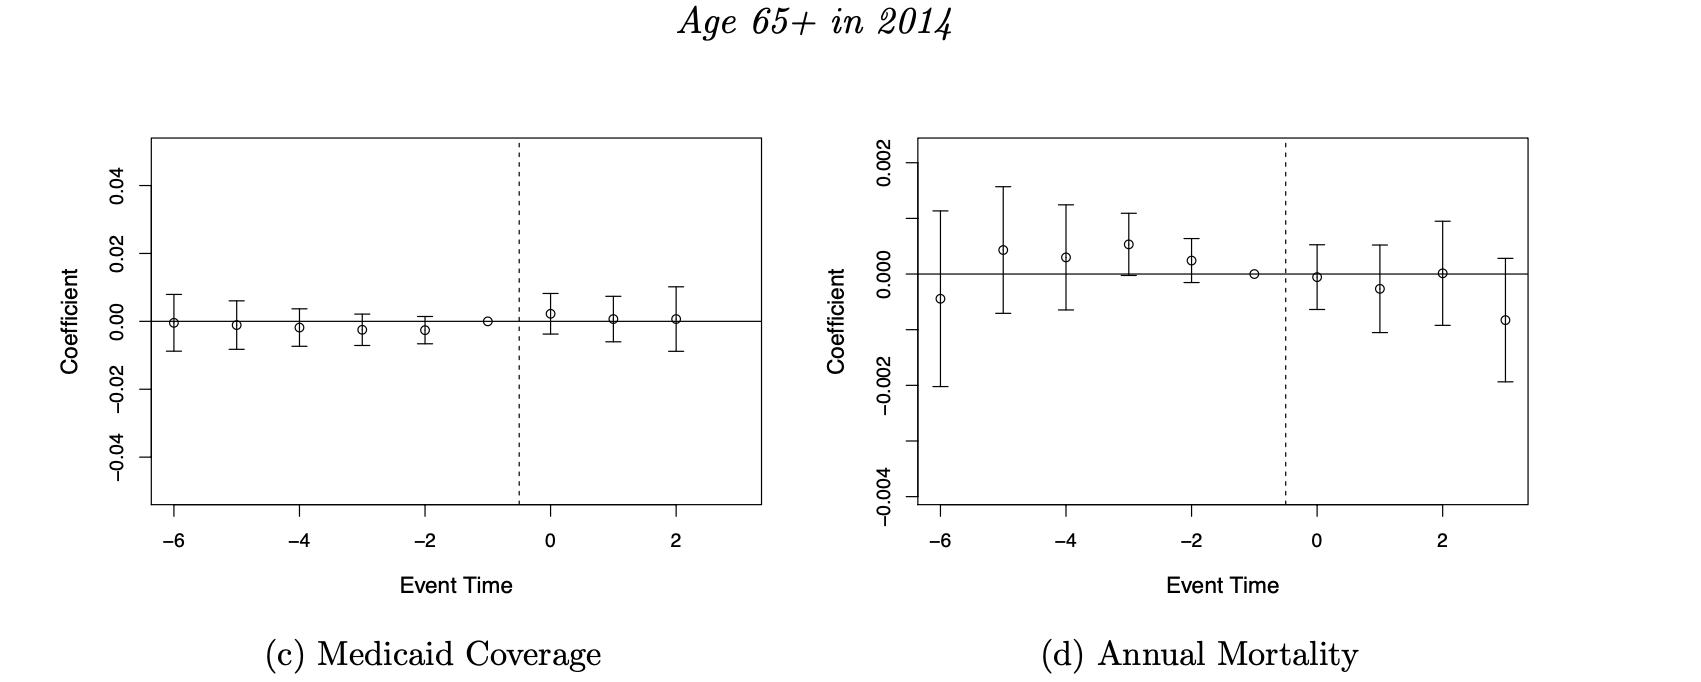
\includegraphics[scale=0.425]{./lecture_includes/placebo_medicaid}
	\end{figure}

\end{frame}



\begin{frame}[plain]

	\begin{figure}
	\includegraphics[scale=0.3]{./lecture_includes/Miller_Medicaid4.png}
	\caption{Miller, et al. (2019) estimates of Medicaid expansion's effects on on annual mortality}
	\end{figure}

\end{frame}

\begin{frame}{Reviewing the evidence}

\begin{itemize}
\item \textbf{Bite}: Increases in enrollment and reductions in uninsured support that there is adoption of the treatment
\item \textbf{Main Results}: 9.2\% reduction in mortality among the near-elderly
\item \textbf{Falsifications}: no effect on a similar group who isn't eligible
\item \textbf{Mechanism}: ``The effect is driven by a reduction in disease-related deaths and grows over time.''
\item \textbf{Event studies}: Compelling once the others are established
\end{itemize}

\end{frame}

\begin{frame}{Making event study}

\begin{itemize}
\item All the simple event study is is an interaction between the treatment group dummy and the calendar year dummies
\item You must drop a $t-\tau$ as the baseline (e.g., $t-1$) must be $Y^0$ untreated comparisons recall
\item I have included in a do file that will do it for you either manually or using coefplot in \texttt{simple\_eventstudy.do} at github labs
\end{itemize}

\end{frame}


\begin{frame}{Manually creating the event study}

	\begin{figure}
	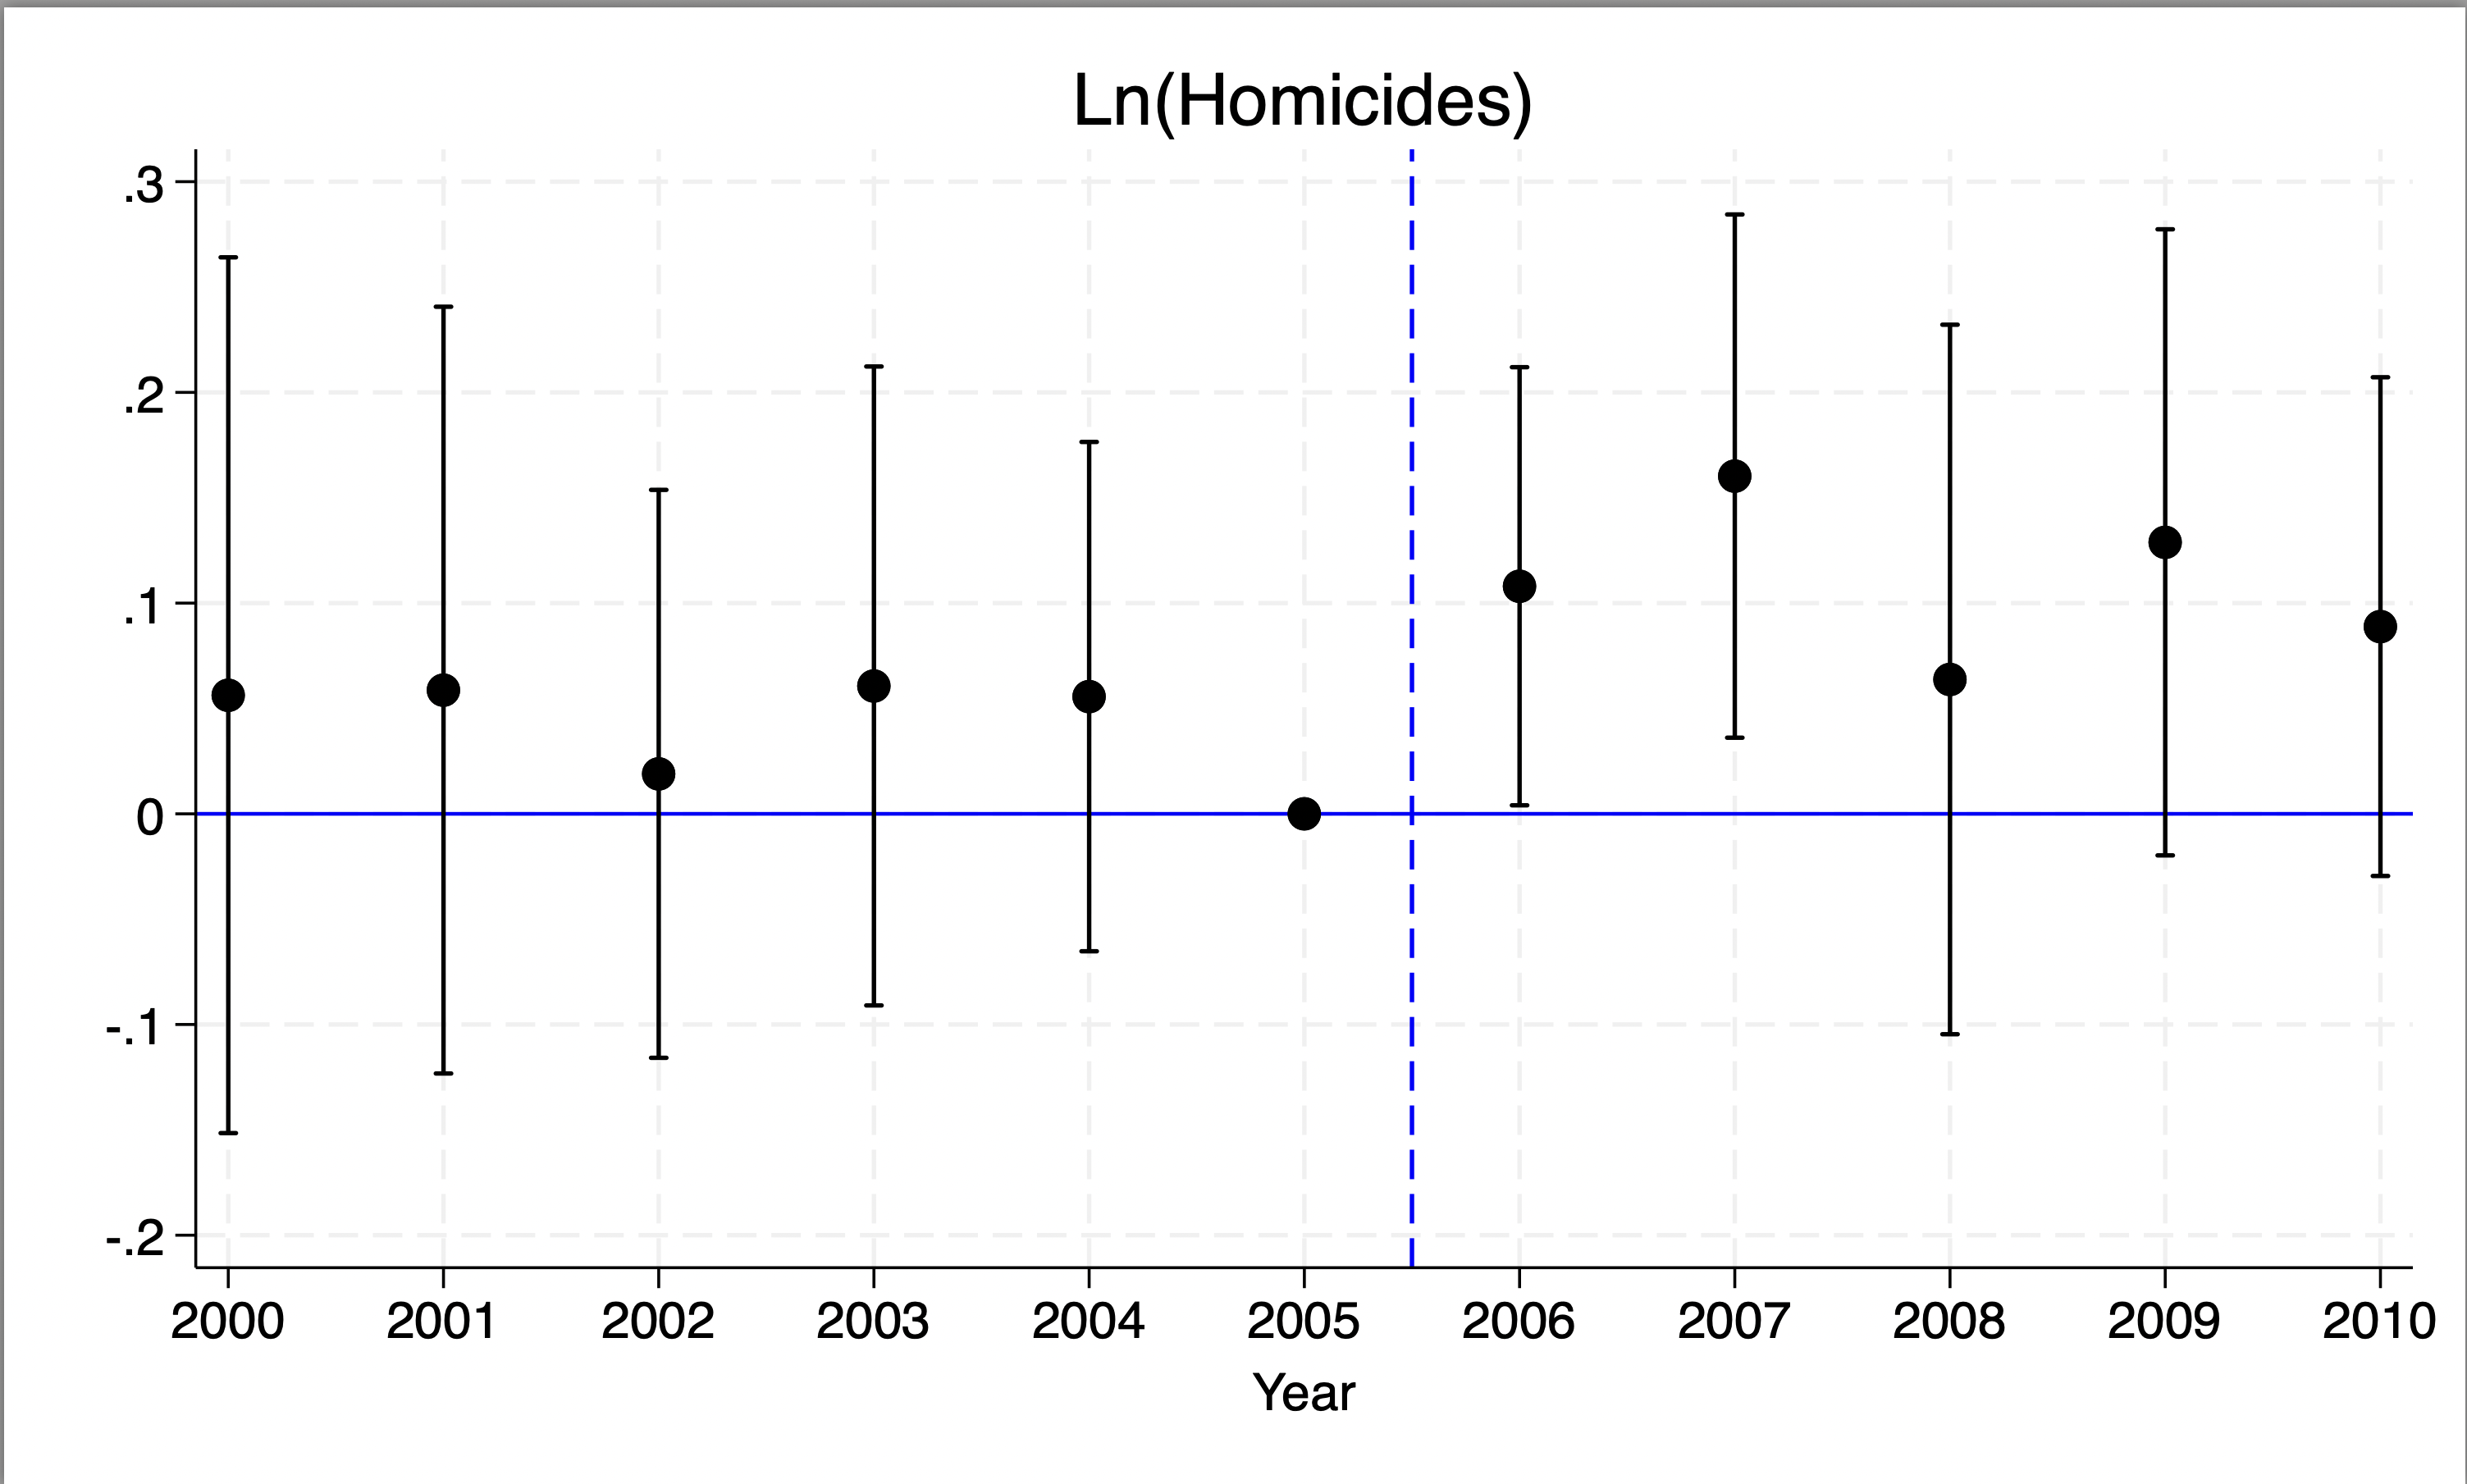
\includegraphics[scale=0.20]{./lecture_includes/simple_eventstudy_manual}
	\end{figure}

\end{frame}




\begin{frame}{Creating the event study with Ben Jann's \texttt{coefplot}}

	\begin{figure}
	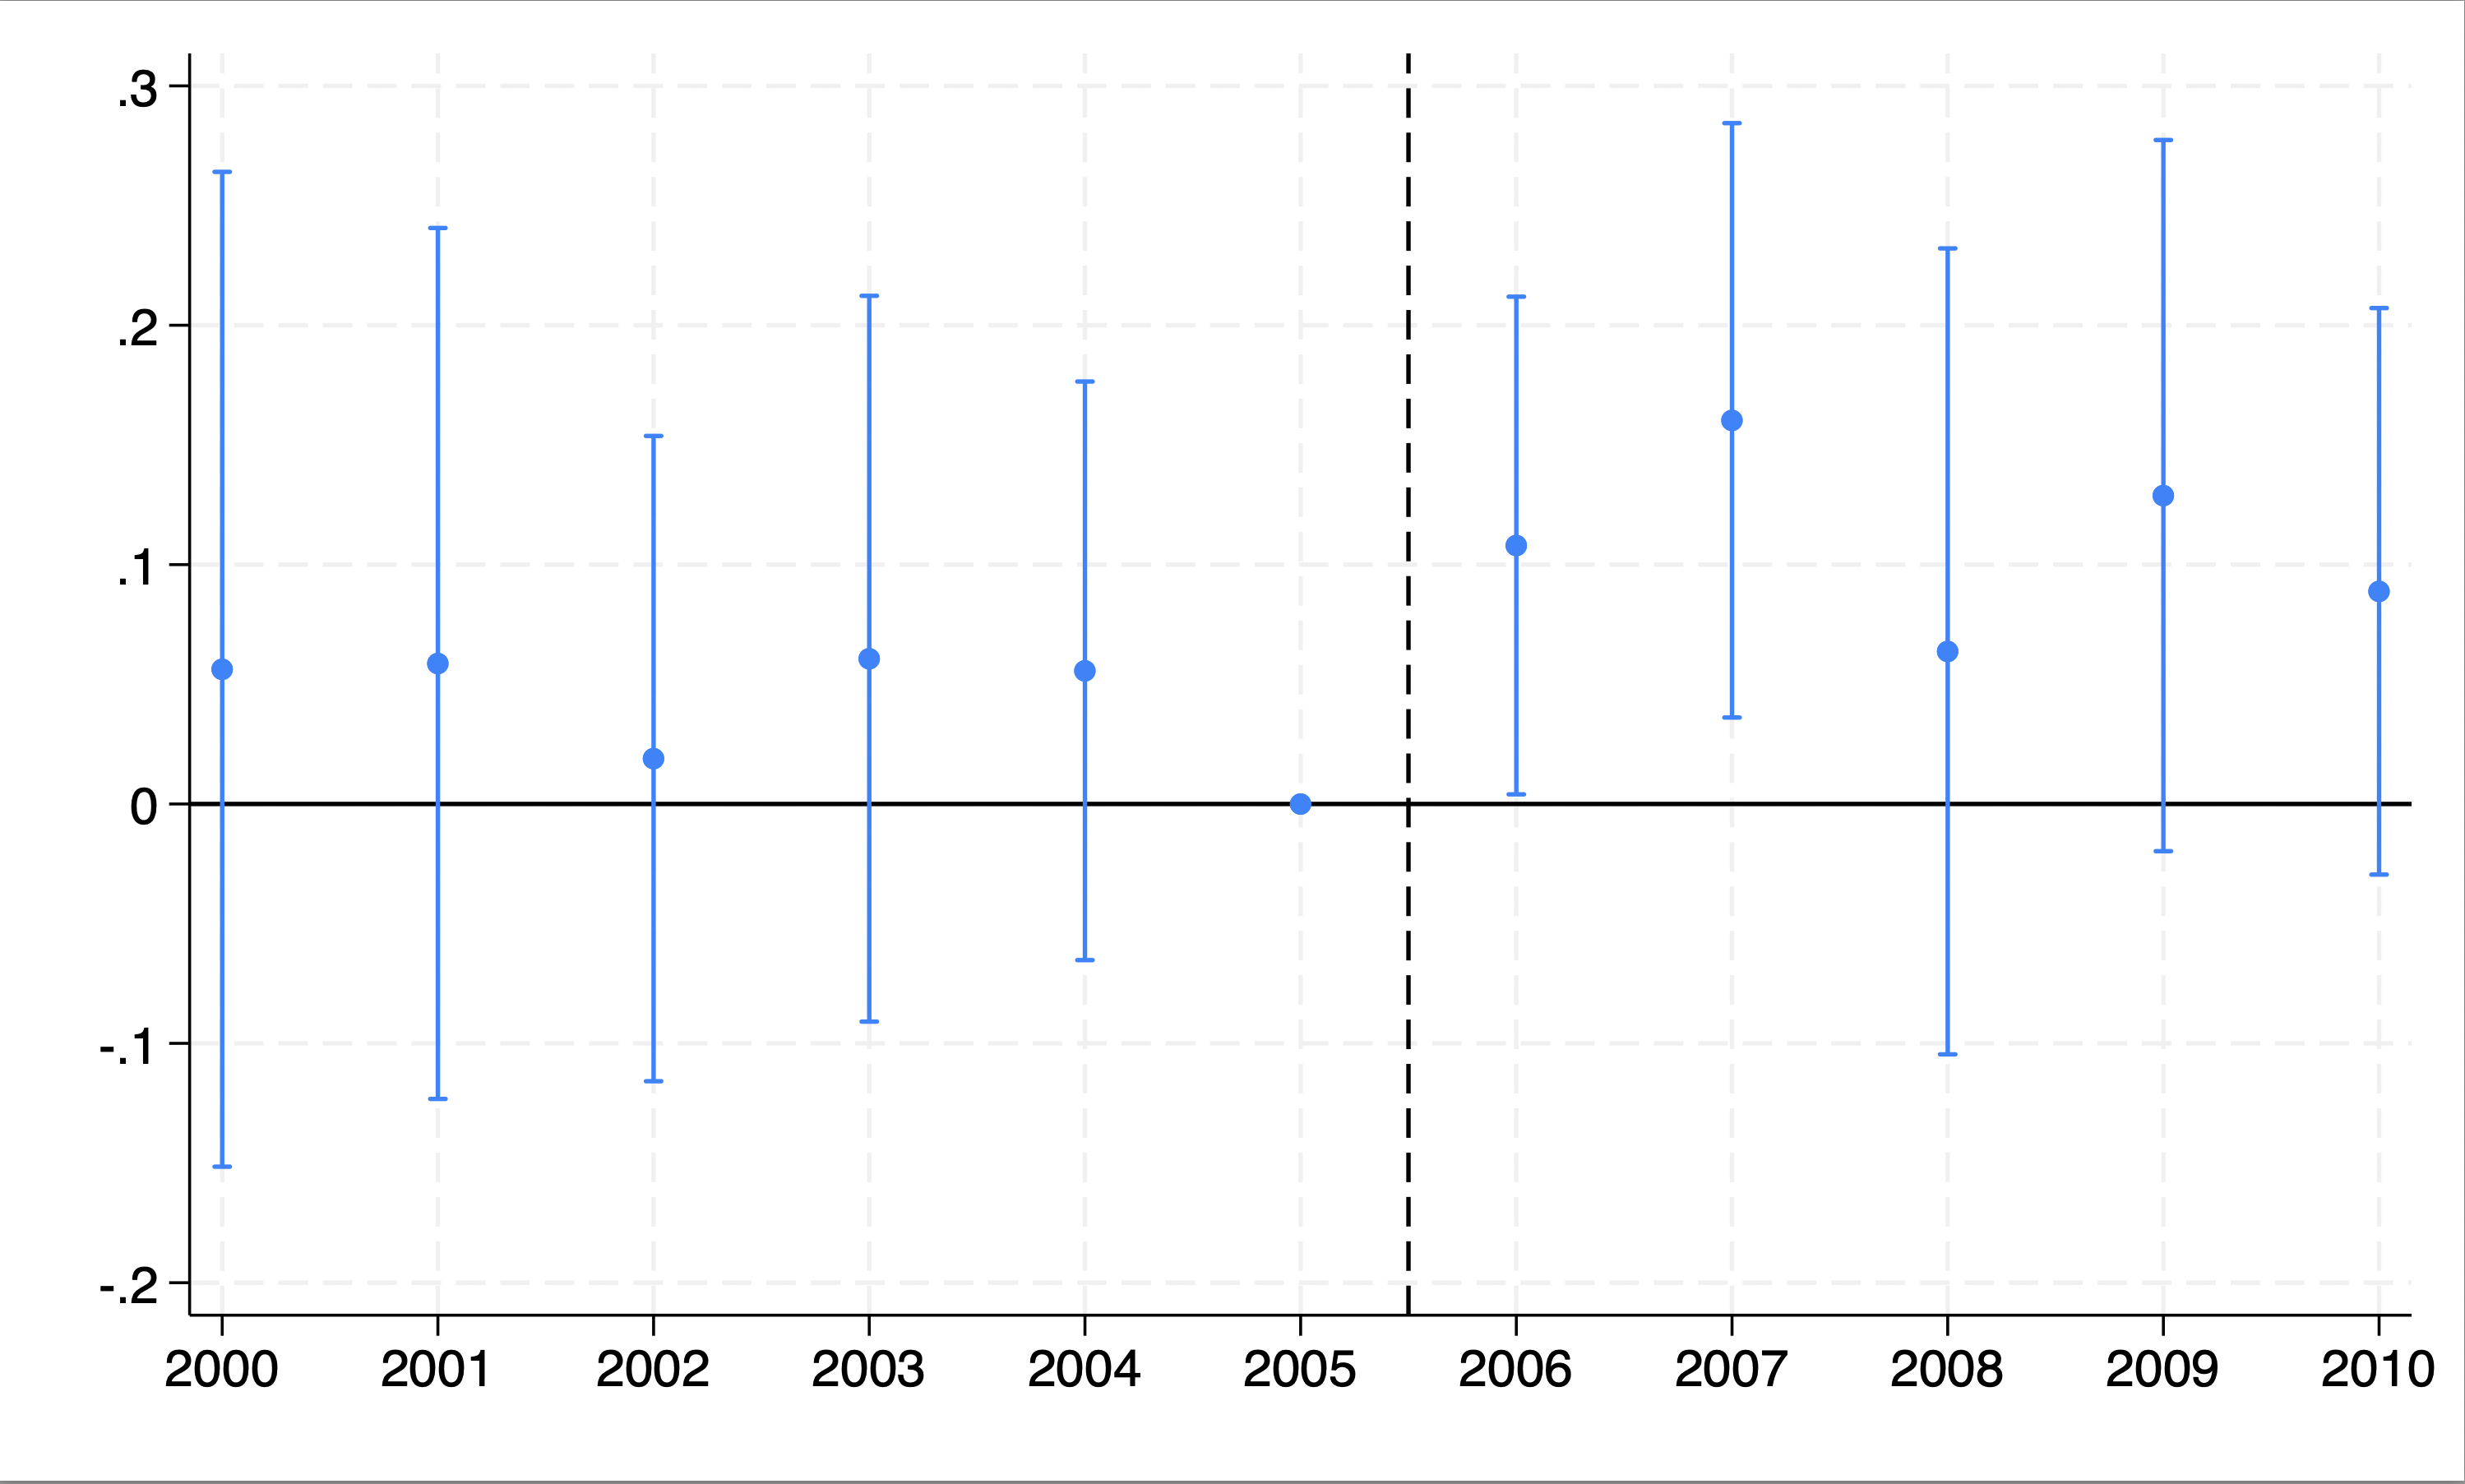
\includegraphics[scale=0.20]{./lecture_includes/simple_eventstudy.png}
	\end{figure}

\end{frame}





\subsection{Falsifications}

\begin{frame}{What are falsifications}

\begin{itemize}
\item Falsifications are indirect evidence that parallel trends probably holds by testing competing hypotheses directly
\item These are outcomes that shouldn't be affected (``falsification on unaffected outcomes'') or groups that shouldn't be affected (``falsification on comparison groups'')
\item Good falsifications require a shared belief they are good falsifications (requires buy-in)
\item Can be hard if you work in an obscure area in which you have deep institutional knowledge but that's the art of the paper
\end{itemize}

\end{frame}


\begin{frame}{Falsifications on more comparison groups}
	
	\begin{itemize}
	\item Very common for readers and others to request a variety of ``robustness checks'' from a DD design
	\item We saw some of these just now (e.g., falsification test using data for alternative control group, the Medicare population)
	\item Triple differences is a formal design based on the idea that another group is unaffected by which is treated with competing forces
	\item Not a true falsification because the diff-in-diff need not be zero -- triple diff has its own parallel trends assumption
	\end{itemize}
\end{frame}

\begin{frame}{Triple differences by Gruber (1995)}
	
	\begin{figure}
	\includegraphics{./lecture_includes/gruber_ddd_3.pdf}
	\end{figure}
	
\end{frame}



\begin{frame}[shrink=20]

\begin{table}\centering
		\caption{Difference-in-Difference-in-Differences numerical example}
		\tiny
		\begin{center}
		\begin{tabular}{lll|l|lll}
		\hline \hline
		\multicolumn{1}{l}{\textbf{States}}&
		\multicolumn{1}{c}{\textbf{Group}}&
		\multicolumn{1}{c}{\textbf{Period}}&
		\multicolumn{1}{c}{\textbf{Outcomes}}&
		\multicolumn{1}{c}{$D_1$}&
		\multicolumn{1}{c}{$D_2$}&
		\multicolumn{1}{c}{$D_3$}\\
		\hline
		&&After	&$\textcolor{red}{NJ+T+NJ_t+w_t+D}$					\\
	&Married women, 20-40yo			&&&$\textcolor{red}{T+NJ_t+w_t+D}$			\\
		&&Before	&$NJ$					\\
Treatment states					&&&&&$\textcolor{red}{D+w_t-m_t}$			\\
		&&After	&$NJ+T+NJ_t+s_t$					\\
	&Single men 20-40yo		&&	&$T+NJ_t+m_t$				\\
		&&Before	&$NJ$					\\
								\\
&&&&&&$\widehat{D}$
\\
		&&After	&$PA+T+PA_t+w_t$				\\
	&Married women, 20-40yo			&&&$T+PA_t+w_t$ \\				
		&&Before	&$PA$					\\
Comparison states					&&&&&$w_t-m_t$		\\
		&&After	&$PA+T+PA_t+m_t$					\\
	&Single men 20-40yo		&&&	$T+PA_t+m_t$				\\
		&&Before	&$PA$					\\
		\hline \hline
		\end{tabular}
		\end{center}
	\end{table}
	
\begin{center}
\textbf{Triple diff estimation and identification:} 
\end{center}

\textbf{Estimation}: Eight averages and seven differences because it's differencing two diff-in-diff

\bigskip

\textbf{Parallel trend assumption}: $\textcolor{red}{w_t-m_t}$ for experimental states equals $\textcolor{black}{w_t-m_t}$ for non-experimental states

\bigskip

\textbf{Intuition}: Whatever the difference in change in wages for men and women in PA, that's the change in wages gap in NJ counterfactual (which we don't know)



\end{frame}


\begin{frame}{DDD in Regression}
	
	\begin{eqnarray*}
	Y_{ijt} &=&\alpha +  \beta_2 \tau_t + \beta_3 \delta_j  + \beta_4 D_i + \beta_5(\delta \times \tau)_{jt} \\
	&& +\ \beta_6(\tau \times D)_{ti} +  \beta_7(\delta \times D)_{ij} +  \textcolor{red}{\beta_8(\delta \times \tau \times  D)_{ijt}}+  \varepsilon_{ijt}
	\end{eqnarray*}
	
	\begin{itemize}
	\item Your panel is now a group $j$ state $i$ (e.g., AR women 1991, AR women 1992, etc.)
	\item Each term is a dummy relative to some baseline (pre), omitted group (men) and treatment state (PA)
	\item Most use DDD by assuming DD for control must be zero, but as we saw, formally it just has its own assumption and that need not be zero
	\item Assumption is that its change is the fictional change of our treated group, just like always
		\end{itemize}
	
\end{frame}

\begin{frame}{Great new paper to learn more}

\begin{figure}
\includegraphics[scale=0.25]{./lecture_includes/olden_moen_2022_ddd.png}
\end{figure}

\end{frame}




\begin{frame}{Falsification on outcomes}
	
	\begin{itemize}
	\item The within-group control group (DDD) is a form of placebo analysis using the same \emph{outcome}
	\item But there are also placebos using a \emph{different} outcome -- but you need a hypothesis of mechanisms to figure out what is in fact a \emph{different outcome}
	\item Figure out what those are, and test them -- finding no effect on placebo outcomes tends to help people your other results interestingly enough
	\item Cheng and Hoekstra (2013) examine the effect of castle doctrine gun laws on non-gun related offenses like grand theft auto and find no evidence of an effect 
	\end{itemize}
\end{frame}



\begin{frame}{Rational addiction as a placebo critique}


Sometimes, an empirical literature may be criticized using nothing more than placebo analysis

\begin{quote}``A majority of [our] respondents believe the literature is a success story that demonstrates the power of economic reasoning.  At the same time, they also believe the empirical evidence is weak, and they disagree both on the type of evidence that would validate the theory and the policy implications. Taken together, this points to an interesting gap.  On the one hand, most of the respondents claim that the theory has valuable real world implications.  On the other hand, they do not believe the theory has received empirical support.''
\end{quote}

\end{frame}

\begin{frame}{Placebo as critique of empirical rational addiction}

\begin{itemize}
	\item Auld and Grootendorst (2004) estimated standard ``rational addiction'' models (Becker and Murphy 1988) on data with milk, eggs, oranges and apples.  
	\item They find these plausibly non-addictive goods are addictive, which casts doubt on the empirical rational addiction models.
\end{itemize}

\end{frame}

\begin{frame}{Placebo as critique of peer effects}

\begin{itemize}
	\item Several studies found evidence for ``peer effects'' involving inter-peer transmission of smoking, alcohol use and happiness tendencies
	\item Christakis and Fowler (2007) found significant network effects on outcomes like obesity
	\item Cohen-Cole and Fletcher (2008) use similar models and data and find similar network ``effects'' for things that \emph{aren't} contagious like acne, height and headaches
	\item Ockham's razor - given social interaction endogeneity (Manski 1993), homophily more likely explanation
\end{itemize}

\end{frame}



\section{Conditional parallel trends with covariates}

\subsection{Inverse probability weighting}

\begin{frame}{Covariates and violations}

\begin{itemize}
\item There is an assumption called ``unconfoundedness'' $$( Y^0, Y^1 ) \perp\!\!\!\perp D | X $$
\item It means that within the dimensions of X (e.g., Asian males aged 45), D is assigned to units independent of their potential outcomes or any combination of them (e.g., treatment effects)
\item It's the basis for running regressions with covariates in order to recover aggregate causal parameters outside of the experiment but it claims that with the inclusion of the covariates, you have isolated a randomized experiment
\item We usually motivate this assumption in diff-in-diff, too, but it is technically not what is going on

\end{itemize}

\end{frame}

\begin{frame}{Why covariates?}

\begin{itemize}

\item The inclusion of covariates in diff-in-diff models is not about trying to find random variation in the treatment within values of the dimension of X
\item It is based on the claim that the inclusion of covariates is necessary to re-establish parallel trends
\item This is itself different than how covariates will be used in synthetic control, too
\end{itemize}

\end{frame}





\begin{frame}{Correcting the missingness problem}

\begin{eqnarray*}
\text{ATT} &=& E[\delta | D=1] \\
&=& E[Y^1-\textcolor{red}{Y^0} | D=1] \\
&=& E[Y^1 | D=1] - \textcolor{red}{E[Y^0|D=1]} \\
&=& E[Y | D=1] - \textcolor{red}{E[Y^0|D=1]} 
\end{eqnarray*}

\bigskip

We were always missing $Y^0$ values for the treatment group units, but parallel trends allowed us to impute it using the change in $[Y^0]|D=0]$ as a guide

\bigskip

But if that trend is not a good guide, then we cannot.  


\end{frame}


\begin{frame}{Conditional parallel trends}

The DiD equation yields:

\begin{eqnarray*}
\widehat{\delta} &=& \bigg ( E[Y_k|Post] - E[Y_k|Pre] \bigg ) - \bigg ( E[Y_U | Post ] - E[ Y_U | Pre] \bigg) \\
&=& \text{ATT} + \text{Non-parallel trends bias}
\end{eqnarray*}

\bigskip

If we believe that conditional on covariates, parallel trends holds, but only within values of $X$, then there are methods we can use that incorporate covariates into the DiD equation and unbiasedness returns

\bigskip 

The inclusion of covariates has particular regression specifications, plus there are alternative methods too, and we will review them

\end{frame}




\begin{frame}{Three covariate DiD papers}

Three papers (though sometimes you see others) about covariate adjustment in DiD:
\begin{enumerate}
\item Abadie (2005) on semiparametric DiD -- reweights the comparison group part of the DID equation using a propensity score based on X
\item Heckman, Ichimura and Todd (1997) on outcome regression uses baseline X and control group only to impute the missing counterfactual $Y^0$ for treatment group units in a DiD equation
\item Sant'Anna and Zhou (2020) is double robust which means the method does both of these at the same time so that you don't have to choose between them
\end{enumerate}

\bigskip

We will discuss both of them and then compare their performance with the more straightforward fixed effects model

\end{frame}



\begin{frame}{Semiparametric DiD}


 Abadie (2005) proposed a model that simply reweights the control group in the DiD equation using a particular specification (``semiparametric'') of the propensity score on pretreatment covariates
 
	\begin{enumerate}
	\item Calculate each unit's ``after minus before'' (DiD equation)
	\item Estimate the conditional probability of treatment based on baseline covariates (propensity score estimation)
	\item Weight the comparison group's DiD equation with the propensity score 
	\end{enumerate}

Remember -- ATT is only missing $Y^0$ for treatment, so we only have to apply weights to the comparison group units

\end{frame}

\begin{frame}{Novel elements of time in Abadie's model}

\begin{itemize}
\item There is only one treatment group so therefore there is only one relevant treatment date, $t$
\item The period prior to treatment is called the baseline, or $b$, period and it is when treated units were not treated 
\item $X_b$ are ``baseline'' covariates meaning the value of $X$ in the pre-treatment period for either the treated or comparison group units
\item Propensity scores are estimated off the $b$ period \emph{only} 
\item Abadie ``throws away'' covariates after treatment because this is all about re-establishing parallel trends which is a \emph{baseline} concept recall
\end{itemize}

\end{frame}

\begin{frame}{Assumptions}

Three main assumptions

\begin{enumerate}
\item Conditional parallel trends $$E[Y^0_t - Y^0_b|D=1,X_b] - E[Y^0_t - Y^0_t | D=0, X_b]$$ 
\item Common support $$Pr(D=1)>0; Pr(D=1|X)<1$$ 
\item Propensity score model is properly specified 
\end{enumerate}

\end{frame}

\begin{frame}{Propensity scores as dimension reduction}

\begin{itemize}

\item Propensity scores are ways of dealing with a conditioning set $X$ that has large dimensions
\item Dimensions are not the same as covariates -- if you have continuous $X$, then it has infinite dimensions
\item Common support means that \emph{within} all combinations of the covariates (e.g., white male 47yo versus whites, males, age) there are units in treatment and control

\end{itemize}

\end{frame}

\begin{frame}{Common support example}

Think of common support like ``exact matches'' but on the propensity score

\bigskip

I'm a white male 47 years old with a PhD; can I find a white male 47 years old without a PhD

\bigskip

If I can, that's common support; if I cannot that's off support

\end{frame}


\begin{frame}{Propensity scores as dimension reduction}

\begin{itemize}

\item Propensity score theorem (Rosenbaum and Rubin 1983) showed that if you need $X$ to satisfy some assumption, the propensity score will satisfy too
\item Propensity scores essentially transform your large dimensional problem into a single scalar called the propensity score, which is the conditional probability of treatment (conditional on $X$)
\item But we need to estimate the propensity score because we don't usually know it (only an experimentalist ``knows'' the true propensity score)

\end{itemize}

\end{frame}

\begin{frame}{Common support and the propensity score}

\begin{itemize}
\item Exact matches mean you have people who are identical on covariate values in both treatment and control
\item Common support and the propensity score means you have people nearly identical on their probability of treatment
\item I am 47yo white male with a PhD with a propensity score of 0.75, but you are an Asian female 27yo without a PhD and have a propensity score of 0.75
\item Same idea, but for this to work, we need to have ``matches'' like that (just on the propensity score)
\end{itemize}

\end{frame}


\begin{frame}{How do these work together?}

Since we are identifying the ATT, and the ATT is missing $Y^0$ for the treated group, we are using the control group $Y^0$ in its place 

\bigskip

Under conditional parallel trends and common support, some of the comparison group units are recovering the parallel trends because of their $X$ values creating projections that in their differences perfectly aligned in expectation with the missing $\Delta E[Y^0|D=1]$

\bigskip

But we have to have all three for it to work

\end{frame}

\begin{frame}{Visualizing propensity score to get common support}

	\begin{figure}
	\includegraphics[scale=0.05]{./lecture_includes/common_support_abadie.png}
	\end{figure}

\end{frame}

\begin{frame}{Definition and estimation}

Defining the ATT parameter of interest
\begin{eqnarray*}
ATT &=& E[Y^1_t - \textcolor{red}{Y^0_t} |D=1] \\
&=&E[Y^1_t  | D = 1 ] - \textcolor{red}{E[Y^0_t | D=1]}
\end{eqnarray*}

\bigskip
Abadie's inverse probability weighting (IPW) estimator
\begin{eqnarray*}
E\bigg [ \frac{Y_t - Y_b}{Pr(D_t=1)} \times \frac{D_t - Pr(D=1|X_b)}{1-Pr(D=1|X_b)} \bigg ]
\end{eqnarray*}

\bigskip

The first is our causal parameter; the second is our reweighted DiD equation that \emph{estimates} our causal parameter, but we need to estimate that propensity score


\end{frame}

\begin{frame}{Abadie's IPW estimator}

Look closely; what happens mathematically when you substitute $D=1$ vs $D=0$?

\begin{eqnarray*}
E\bigg [ \frac{Y_t - Y_b}{Pr(D_t=1)} \times \frac{D_t - Pr(D=1|X_b)}{1-Pr(D=1|X_b)} \bigg ]
\end{eqnarray*}

\bigskip

The reweighting with the propensity only happens to the comparison group's first differences -- not the treatment groups!  Why?  Because it's the $Y^0$ that is missing, not the $Y^1$

\end{frame}



\begin{frame}{Propensity scores}

\begin{itemize}
\item It's common to hear people say that we don't know the propensity score; we can only estimate it. Same here -- we approximate it with regressions
\item Paper is titled ``Semi-parametric DiD'' because Abadie imposes structure on the polynomials used to construct the propensity score (``series logit'')
\end{itemize}

\end{frame}



\begin{frame}{Abadie 2005 influence}

	\begin{figure}
	\includegraphics[scale=0.25]{./lecture_includes/abadie_restud_ipw}
	\end{figure}Abadie (2005) is his fourth most cited paper

\end{frame}




\subsection{Outcome Regression and Double Robust}

\begin{frame}{Outcome Regression Paper}

	\begin{figure}
	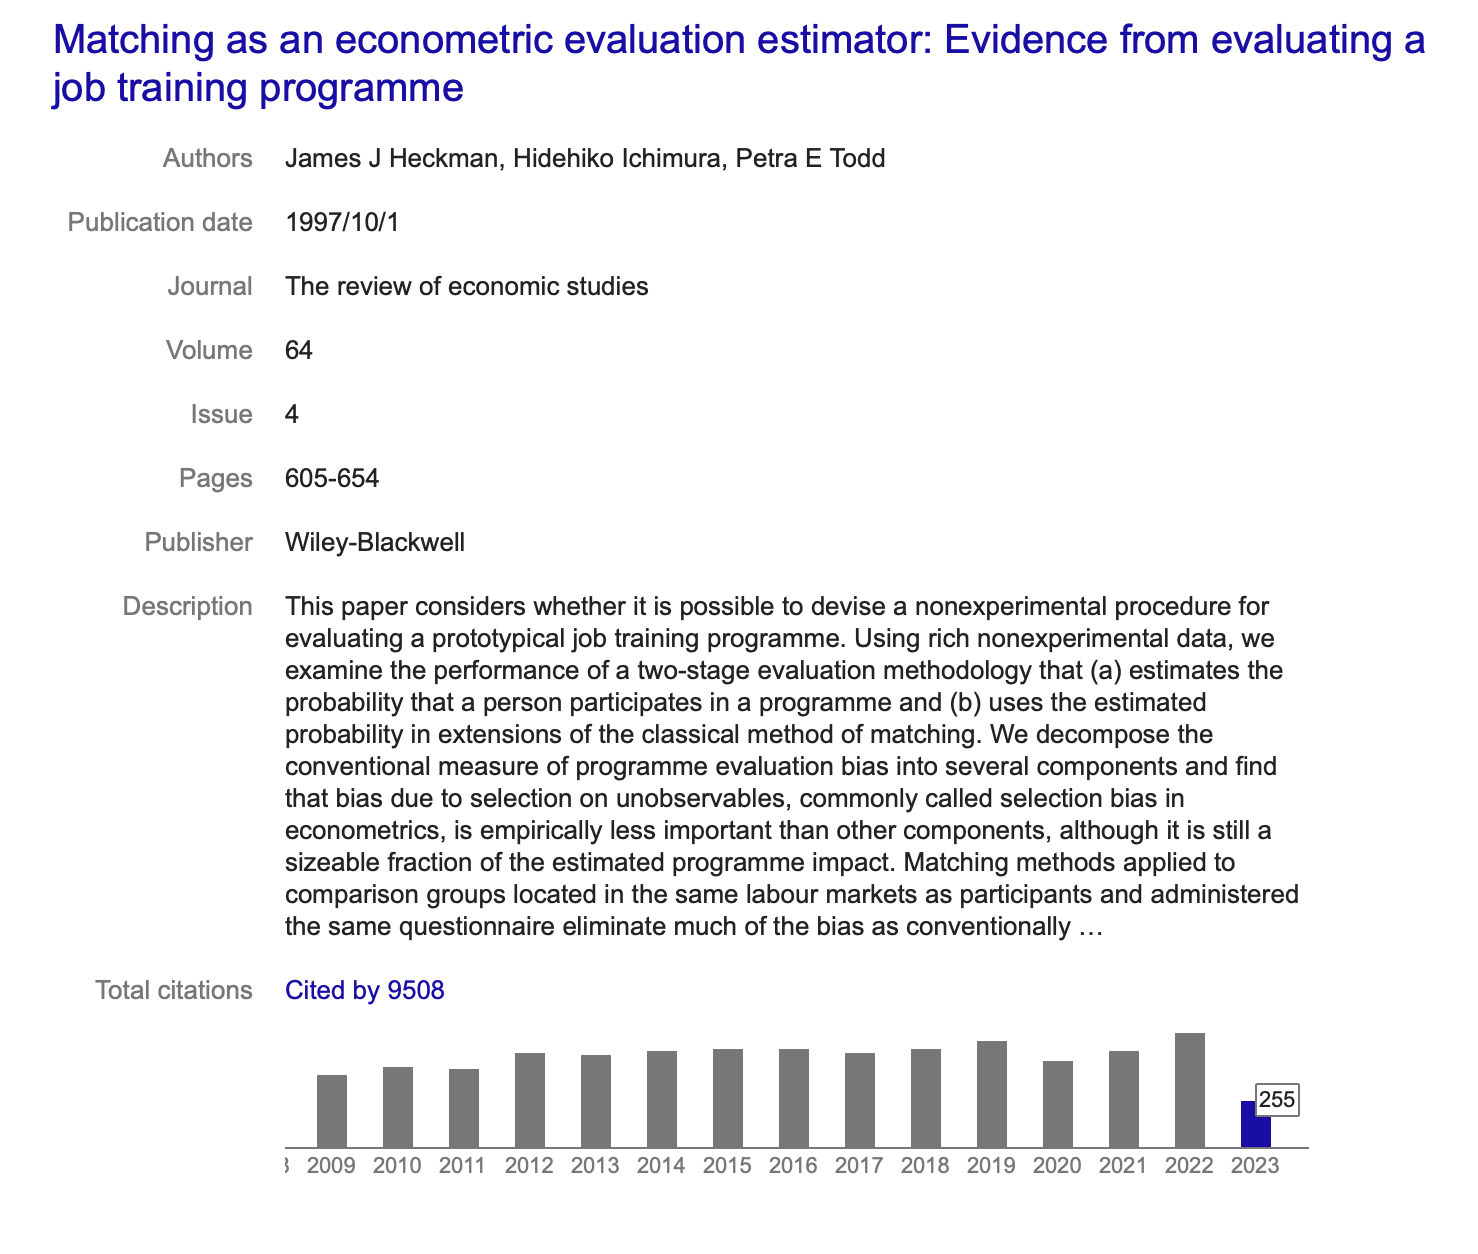
\includegraphics[scale=0.25]{./lecture_includes/or_cites}
	\end{figure}Heckman, Ichimura and Todd (1997) is Petra and Hide's most cited paper and Heckman's second most cited!

\end{frame}



\begin{frame}{Doubly Robust Paper}

	\begin{figure}
	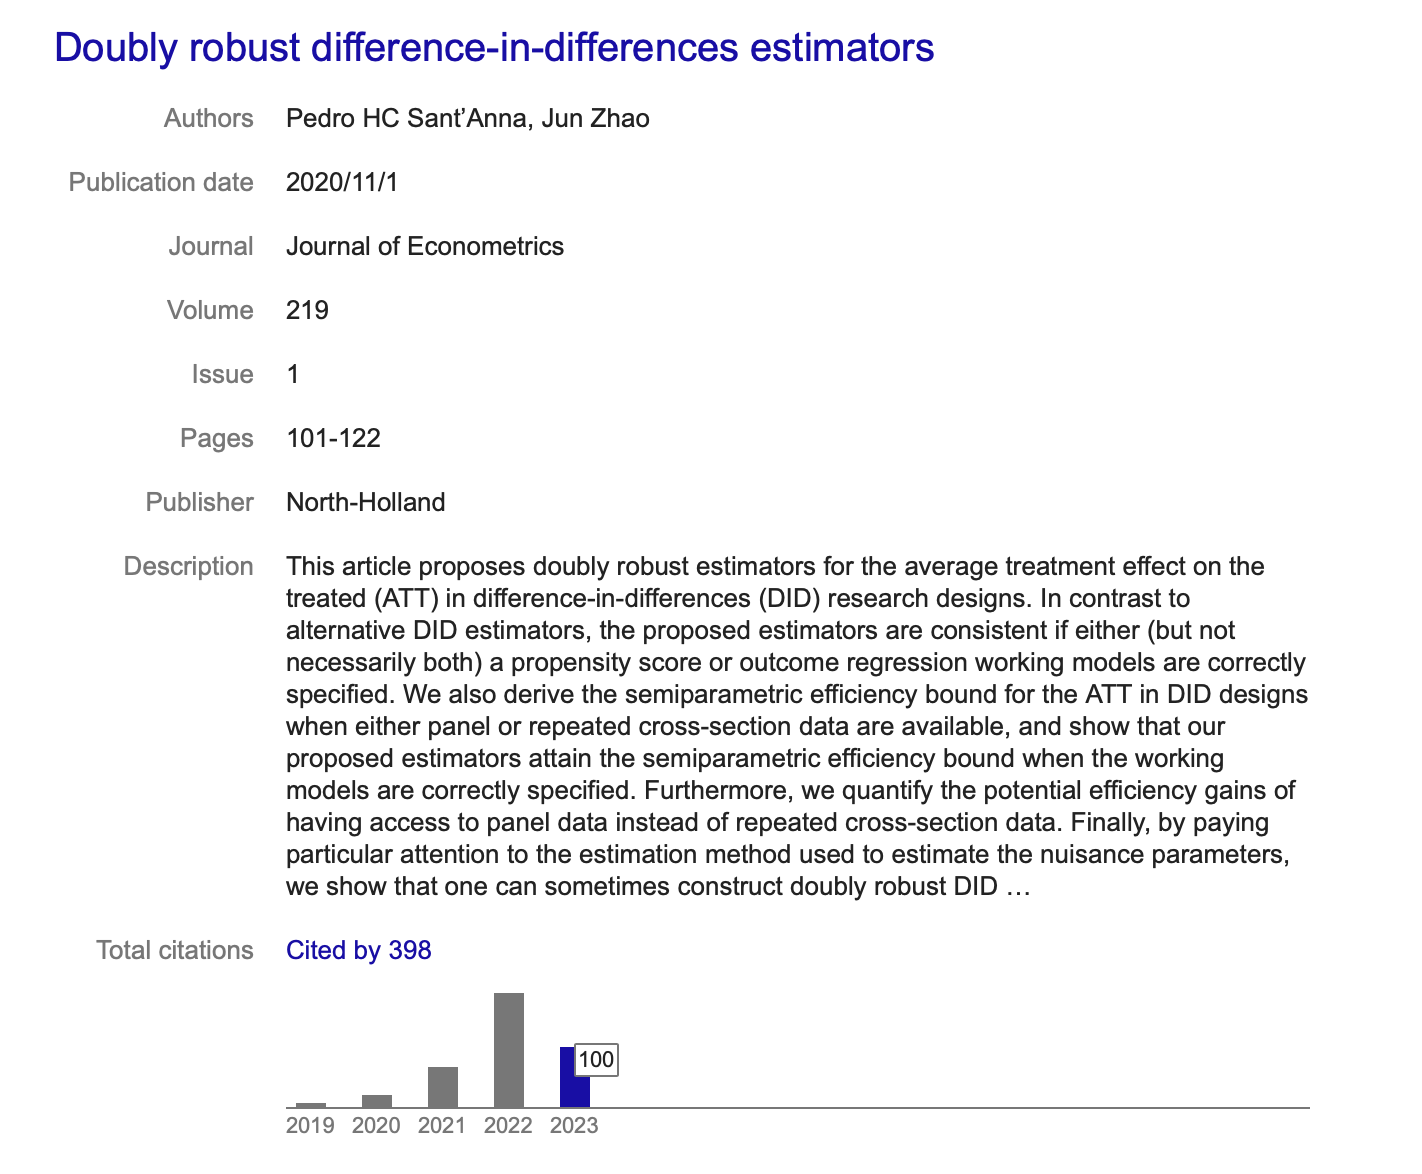
\includegraphics[scale=0.25]{./lecture_includes/pedro_dr_cites}
	\end{figure}Sant'Anna and Zhao (2020) is Pedro's second most cited paper

\end{frame}




\begin{frame}{Doubly Robust Difference-in-differences}

\begin{itemize}
\item DR models control for covariates twice -- once using the propensity score, once using outcomes adjusted by regression -- and are unbiased so long as:
	\begin{itemize}
	\item The regression specification for the outcome is correctly specified
	\item The propensity score specification is correctly specified
	\end{itemize}
\item Sant'Anna and Zhao (2020) incorporated DR into DiD by combining inverse probability weighting and outcome regression into a single DiD model
\item It's in the engine of Callaway and Sant'Anna (2020) that we discuss later so it merits close study
\end{itemize}

\end{frame}




\begin{frame}{Identification assumptions I: Data}

Assumption 1: Assume panel data or repeated cross-sectional data

\bigskip

Handling repeated cross-sectional data is possible but assumes stationarity which is a kind of stability assumption, but I'll use panel representation. 

\bigskip

Cross-sections will be potentially violated with changing sample compositions (e.g., the Napster example). 

\end{frame}

\begin{frame}{Identification assumptions II: Modification to parallel trends}

Assumption 2: Conditional parallel trends

\bigskip

Counterfactual trends for the treatment group are the same as the control group for all values of $X$

\begin{eqnarray*}
E[Y_1^0 - Y_0^0 | X, D=1] = E[Y^0_1 - Y^0_0 | X, D=0]
\end{eqnarray*}

\end{frame}

\begin{frame}{Identification assumptions III: Common support}

Assumption 3: Common support

\bigskip

For some $e>0$, the probability of being in the treatment group is greater than $e$ and the probability of being in the treatment group conditional on $X$ is $\leq1-e$. 

\bigskip

Heckman, et al doesn't use the propensity score so we need a more general expression of support

\end{frame}

\begin{frame}{Estimating DD with Assumptions 1-3}

\begin{itemize}
\item Assumptions 1-3 gives us a couple of options of estimating the DiD
\item We can either use the outcome regression (OR) approach of Heckman, et al 1997 (will require correct model too)
\item Or we can use the inverse probability weighting (IPW) approach of Abadie (2005) (will require correct model too)
\end{itemize}

\end{frame}



\begin{frame}{Outcome regression}

This is the Heckman, et al. (1997) approach where the potential outcome evolution for the treatment group is imputed with a regression based only on $X_b$ for the control group \emph{only}

\bigskip

\begin{eqnarray*}
\widehat{\delta}^{OR} = \overline{Y}_{1,1} - \bigg [ \overline{Y}_{1,0} + \frac{1}{n^T} \sum_{i|D_i=1} ( \widehat{\mu}_{0,1}(X_i) - \widehat{\mu}_{0,0}(X_i)) \bigg ]
\end{eqnarray*}

where $\overline{Y}$ is the sample average of $Y$ among units in the treatment group at time $t$ and $\widehat{\mu}(X)$ is an estimator of the true, but unknown, $m_{d,t}(X)$ which is by definition equal to $E[Y_t|D=d,X=x]$.

\end{frame}




\begin{frame}{Outcome regression}

\begin{eqnarray*}
\widehat{\delta}^{OR} = \overline{Y}_{1,1} - \bigg [ \overline{Y}_{1,0} + \frac{1}{n^T} \sum_{i|D_i=1} ( \widehat{\mu}_{0,1}(X_i) - \widehat{\mu}_{0,0}(X_i)) \bigg ]
\end{eqnarray*}

\begin{enumerate}
\item Regress changes $\Delta Y$ on $X$ among untreated groups using baseline covariates only
\item Get fitted values of the regression using all $X$ from $D=1$ only.  Average those
\item Calculate change in this fitted $Y$ among treated with the average fitted values
\end{enumerate}

\end{frame}

\begin{frame}{Inverse probability weighting}

This is the Abadie (2005) approach where we use weighting

\begin{eqnarray*}
\widehat{\delta}^{ipw} = \frac{1}{E_N[D]} E \bigg [ \frac{D-\widehat{p}(X)}{1-\widehat{p}(X)} (Y_1-Y_0) \bigg ]
\end{eqnarray*}

where $\widehat{p}(X)$ is an estimator for the true propensity score. Reduces the dimensionality of $X$ into a single scalar.

\end{frame}

\begin{frame}{These models cannot be ranked}

\begin{itemize}
\item Outcome regression needs $\widehat{\mu}(X)$ to be correctly specified, whereas
\item Inverse probability weighting needs $\widehat{p}(X)$ to be correctly specified
\item It's hard to ``rank'' these two in practice with regards to model misspecification because each is inconsistent when their own models are misspecified
\end{itemize}

\end{frame}


\begin{frame}{TWFE}

Consider our earlier TWFE specification:

\begin{eqnarray*}
Y_{it} = \alpha_1  + \alpha_2 T_t + \alpha_3 D_i +  \delta (T_i \times D_t)  + \varepsilon_{it}
\end{eqnarray*}

\bigskip

Just add in covariates then right?

\begin{eqnarray*}
Y_{it} = \alpha_1  + \alpha_2 T_t + \alpha_3 D_i  + \delta (T_i \times D_t) + \theta \cdot X_{it} + \varepsilon_{it}
\end{eqnarray*}

Sure! If you're willing to impose three \emph{more} assumptions

\end{frame}




\begin{frame}{Decomposing TWFE with covariates}

TWFE places restrictions on the DGP. Previous TWFE regression under assumptions 1-3 implies the following:

\bigskip

\begin{eqnarray*}
E[Y^1_1|D=1,X] = \alpha_1 + \alpha_2 + \alpha_3 + \delta + \theta X
\end{eqnarray*}

\bigskip

Conditional parallel trends implies

\small
\begin{eqnarray*}
&&E[Y^0_{1} - Y^0_{0}|D=1,X]= E[Y^0_{1} - Y^0_{0}|D=0,X] \\
&&E[Y^0_{1}|D=1,X] - E[Y^0_{0}|D=1,X]= E[Y^0_{1}|D=0,X] - E[Y^0_{0}|D=0,X] \\
&&E[Y^0_{1}|D=1,X] = E[Y^0_{0}|D=1,X] + E[Y^0_{1}|D=0,X] - E[Y^0_{0}|D=0,X] \\
&&E[Y^0_{1}|D=1,X] = E[Y_{0}|D=1,X] + E[Y_{1}|D=0,X] - E[Y_{0}|D=0,X] \\
\end{eqnarray*}


\end{frame}

\begin{frame}{Switching equation substitution}

Last line from the switching equation. This gives us:

\begin{eqnarray*}
E[Y^0_{1}|D=1,X] = \alpha_1  + \alpha_2 + \alpha_3 + \theta X
\end{eqnarray*}

Now compare this with our earlier $Y^1$ expression

\begin{eqnarray*}
E[Y^1_1|D=1,X] = \alpha_1 + \alpha_2 + \alpha_3 + \delta + \theta X
\end{eqnarray*}

We can define our target parameter, the ATT, now in terms of the fixed effects representation

\end{frame}


\begin{frame}{Collecting terms}

TWFE representation of our conditional expectations of the potential outcomes
\begin{eqnarray*}
&&E[Y^1_1|D=1,X] = \alpha_1 + \alpha_2 + \alpha_3 + \delta + \theta_1 X \\
&&E[Y^0_{1}|D=1,X] = \alpha_1  + \alpha_2 + \alpha_3 + \theta_2 X \\
\end{eqnarray*}

Substitute these into our target parameter

\begin{eqnarray*}
ATT &=& E[Y^1_1|D=1,X]  - E[Y^0_{1}|D=1,X]   \\
&&=(\alpha_1 + \alpha_2 + \alpha_3 + \delta + \theta_1 X) - ( \alpha_1  + \alpha_2 + \alpha_3 + \theta_2 X )\\
&&=\delta + (\theta_1 X - \theta_2 X)
\end{eqnarray*}

\bigskip

What if $\theta_1 X \neq \theta_2 X$?

\end{frame}

\begin{frame}{Assumption 4: Homogeneous treatment effects in X}


TWFE requires homogenous treatment effects in $X$ (i.e., the treatment effect is the same for all $X$)

\bigskip

If $X$ is sex, then effects are the same for males and females.

\bigskip

  If $X$ is continuous, like income, then the effect is the same whether someone makes \$1 or \$1 million.

\end{frame}

\begin{frame}{X-specific trends}

TWFE also places restrictions on covariate trends for the two groups too.  Take conditional expectations of our TWFE equation. 

\begin{eqnarray*}
E[Y_1|D=1] &=& \alpha_1 + \alpha_2 + \alpha_3 + \delta + \theta X_{11} \\
E[Y_0|D=1] &=& \alpha_1 + \alpha_3 + \theta X_{10} \\
E[Y_1|D=0] &=& \alpha_1 + \alpha_2 + \theta X_{01} \\
E[Y_0|D=0] &=& \alpha_1 + \theta X_{00}
\end{eqnarray*}


\end{frame}


\begin{frame}{X-specific trends}

Now take the DiD formula:

\begin{eqnarray*}
\delta^{DD} = &&\bigg ( (\alpha_1 + \alpha_2 + \alpha_3 + \delta + \theta X_{11} ) - (\alpha_1 + \alpha_3 + \theta X_{10} ) \bigg )- \\
&& \bigg ( (\alpha_1 + \alpha_2 + \theta X_{01}) - (\alpha_1 + \theta X_{00}) \bigg )
\end{eqnarray*}

\bigskip

Eliminating terms, we get:

\begin{eqnarray*}
\delta^{DD} = &&\delta + \\
&& (\theta X_{11} - \theta X_{10} ) - (\theta X_{01} - \theta X_{00} )
\end{eqnarray*}

\bigskip

Second line requires that trends in X for treatment group equal trends in X for control group.

\end{frame}


\begin{frame}{Assumption 5 and 6}

We need ``no X-specific trends'' for the treatment group (assumption 5) and comparison group (assumption 6)

\bigskip

\textbf{Intuition}: No X-specific trends means the evolution of potential outcome $Y^0$ is the same regardless of $X$. This would mean you cannot allow rich people to be on a different trend than poor people, for instance.

\bigskip

Without these six, in general TWFE will not identify ATT. 

\end{frame}

\begin{frame}{Why not both?}

\begin{itemize}
\item Let's review the problem.  What if you claim you need $X$ for conditional parallel trends?
\item You have three options:
	\begin{enumerate}
	\item Outcome regression (Heckman, et al. 1997) -- needs Assumptions 1-3
	\item Inverse probability weighting (Abadie 2005) -- needs Assumptions 1-3
	\item TWFE (everybody everywhere all the time) -- needs Assumptions 1-6
	\end{enumerate}
\item Problem is 1 and 2 need the models to be correctly specified
\item Doubly robust combines them to give us insurance; we now get two chances to be wrong, as opposed to just one
\end{itemize}

\end{frame}


\begin{frame}{Double Robust DiD}
\begin{eqnarray*}
\delta^{dr} = E \bigg [ \bigg ( \frac{D}{E[D]} -\frac{ \frac{p(X)(1-D)}{(1-p(X))} }{E \bigg [\frac{p(X)(1-D)}{(1-p(X))} \bigg ]} \bigg  )( \Delta Y - \mu_{0,\Delta}(X)) \bigg ]
\end{eqnarray*}

\begin{eqnarray*}
&&p(x): \text{propensity score model} \\
&& \Delta Y = Y_1 - Y_0 = Y_{post} - Y_{pre} \\
&& \mu_{d,\Delta} = \mu_{d,1}(X) - \mu_{d,0}(X), \text{ where } \mu(X) \text{ is a model for} \\
&& m_{d,t} = E[Y_t|D=d,X=x]
\end{eqnarray*}So that means $\mu_{0,\Delta}$ is just the control group's change in average $Y$ for each $X=x$

\end{frame}

\begin{frame}{Double Robust DiD}

\begin{eqnarray*}
\delta^{dr} = E \bigg [ \bigg ( \frac{D}{E[D]} -\frac{ \frac{p(X)(1-D)}{(1-p(X))} }{E \bigg [\frac{p(X)(1-D)}{(1-p(X))} \bigg ]} \bigg  )( \Delta Y - \mu_{0,\Delta}(X)) \bigg ]
\end{eqnarray*}

Notice how the model controls for $X$: you're weighting the adjusted outcomes using the propensity score

\bigskip

The reason you control for $X$ twice is because you don't know which model is right.  DR DiD frees you from making a choice without making you pay too much for it


\end{frame}

\begin{frame}{Efficiency}

\begin{itemize}
\item Authors exploit all the restrictions implied by the assumptions to construct semiparametric bounds
\item This is where the influence function comes in, which those who have studied the DID code closely may have noticed
\item One of the main results of the paper is that the DR DiD estimator is also DR for inference
\item Let's skip to Monte Carlos
\end{itemize}

\end{frame}

\begin{frame}{Monte Carlo details}

\begin{itemize}
\item Compare DR with TWFE, OR and IPW
\item Sample size is 1,000
\item 10,000 Monte Carlo experiments
\item Propensity score estimated with logit; OR estimated using linear specification
\end{itemize}

\end{frame}



\begin{frame}[plain]

\begin{table}[htbp]\centering
\scriptsize
\caption{Monte Carlo Simulations, DGP1, Both OR and Propensity score correct}
\centering
\begin{threeparttable}
\begin{tabular}{l*{5}{c}}
\toprule
\multicolumn{1}{l}{\textbf{}}&
\multicolumn{1}{c}{\textbf{Bias}}&
\multicolumn{1}{c}{\textbf{RMSE}}&
\multicolumn{1}{c}{\textbf{SE}}&
\multicolumn{1}{c}{\textbf{Coverage}}&
\multicolumn{1}{c}{\textbf{CI length}}\\
\midrule
TWFE & -20.9518 & 21.1227 & 2.5271 & 0.000 & 9.9061 \\
OR & -0.0012 & 0.1005 & 0.1010 & 0.9500 & 0.3960 \\
IPW & 0.0257 & 2.7743 & 2.6636 & 0.9518 & 10.4412 \\
DR & -0.0014 & 0.1059 & 0.1052 & 0.9473 & 0.4124 \\
\bottomrule
\end{tabular}
\end{threeparttable}
\end{table}

\end{frame}


\begin{frame}[plain]
	\begin{figure}
	\includegraphics[scale=0.25]{./lecture_includes/mc_dr_1.png}
	\end{figure}

\end{frame}


\begin{frame}[plain]

\begin{table}[htbp]\centering
\scriptsize
\caption{Monte Carlo Simulations, DGP4, Neither OR and Propensity score correct}
\centering
\begin{threeparttable}
\begin{tabular}{l*{5}{c}}
\toprule
\multicolumn{1}{l}{\textbf{}}&
\multicolumn{1}{c}{\textbf{Bias}}&
\multicolumn{1}{c}{\textbf{RMSE}}&
\multicolumn{1}{c}{\textbf{SE}}&
\multicolumn{1}{c}{\textbf{Coverage}}&
\multicolumn{1}{c}{\textbf{CI length}}\\
\midrule
TWFE & -16.3846 & 16.5383 & 3.6268 & 0.000 & 14.2169 \\
OR & -5.2045 & 5.3641 & 1.2890 & 0.0145 & 5.0531 \\
IPW & -1.0846 & 2.6557 & 2.3746 & 0.9487 & 9.3084 \\
DR & -3.1878 & 3.4544 & 1.2946 & 0.3076 & 5.0749 \\
\bottomrule
\end{tabular}
\end{threeparttable}
\end{table}

\end{frame}

\begin{frame}[plain]
	\begin{figure}
	\includegraphics[scale=0.12]{./lecture_includes/mc_dr_2.png}
	\end{figure}


\end{frame}

\subsection{Lalonde lab}

\begin{frame}{R and Stata Code}

There is code in R and Stata (all DiD estimators are now beautifully arranged at a website hosted by Asjad Naqvi)
\begin{itemize}
\item Stata: \textbf{drdid}
\item R: \textbf{drdid}
\end{itemize}

\bigskip

\url{https://asjadnaqvi.github.io/DiD/docs/01_stata/}

\bigskip

Remember -- it's for 2x2 with covariates (i.e., one treatment group). 

\end{frame}

\begin{frame}{Application using real data}

\begin{itemize}
\item Let's now use a real example with real data and see how well this does
\item Famous paper in AER by Lalonde (1986), an Orley and Card student at Princeton
\item Found that most program evaluation did badly, but let's revisit it with diff-in-diff
\end{itemize}

\end{frame}

\begin{frame}{Description of NSW Job Trainings Program}
	
The National Supported Work Demonstration (NSW), operated by Manpower Demonstration Research Corp in the mid-1970s:
	\begin{itemize}
	\item was a temporary employment program designed to help disadvantaged workers lacking basic job skills move into the labor market by giving them work experience and counseling in a sheltered environment
	\item was also unique in that it \textbf{randomly assigned} qualified applicants to training positions:
		\begin{itemize}
		\item \textbf{Treatment group}: received all the benefits of NSW program
		\item \textbf{Control group}: left to fend for themselves
		\end{itemize}
	\item admitted AFDC females, ex-drug addicts, ex-criminal offenders, and high school dropouts of both sexes
	\end{itemize}
\end{frame}

\begin{frame}{NSW Program}
	
	\begin{itemize}
	\item Treatment group members were:
		\begin{itemize}
		\item guaranteed a job for 9-18 months depending on the target group and site
		\item divided into crews of 3-5 participants who worked together and met frequently with an NSW counselor to discuss grievances and performance
		\item paid for their work
		\end{itemize}
	\item Control group members were randomized so the same
	\item Note: the randomization balanced observables and unobservables across the two arms, thus enabling the estimation of an ATE for the people who self-selected into the program
	\end{itemize}
\end{frame}

\begin{frame}{NSW Program}

\begin{itemize}
	\item Other details about the NSW program:
		\begin{itemize}
		\item \underline{Wages}:  NSW offered the trainees lower wage rates than they would've received on a regular job, but allowed their earnings to increase for satisfactory performance and attendance
		\item \underline{Post-treatment}: after their term expired, they were forced to find regular employment
		\item \underline{Job types}:  varied within sites -- gas station attendant, working at a printer shop -- and males and females were frequently performing different kinds of work
		\end{itemize}
\end{itemize}

\end{frame}
	
\begin{frame}{NSW Data}
	
	\begin{itemize}
	\item \underline{NSW data collection}:
		\begin{itemize}
		\item MDRC collected earnings and demographic information from both treatment and control at baseline and every 9 months thereafter
		\item Conducted up to 4 post-baseline interviews
		\item Different sample sizes from study to study can be confusing, but has simple explanations
		\end{itemize}
	\end{itemize}
\end{frame}
	

\begin{frame}{NSW Data}

\begin{itemize}
	\item \underline{Estimation}:
		\begin{itemize}
		\item NSW was a randomized job trainings program; therefore estimating the average treatment effect is straightforward:
			\begin{eqnarray*}
			\frac{1}{N_t}\sum_{D_i=1}Y_i - \frac{1}{N_c}\sum_{D_i=0}Y_i \approx E[Y^1-Y^0] 
			\end{eqnarray*}in large samples assuming treatment selection is independent of potential outcomes (randomization) -- i.e., $(Y^0,Y^1)\independent{D}$. 
		\end{itemize}
	\item \underline{NSW worked}: Treatment group participants' real earnings post-treatment (1978) was positive and economically meaningful -- $\approx$ \$900 (LaLonde 1986) to \$1,800 (Dehejia and Wahba 2002) depending on the sample used
\end{itemize}

\end{frame}
	
\begin{frame}[plain]
	\begin{center}
	LaLonde, Robert J. (1986). \myurlshort{http://business.baylor.edu/scott_cunningham/teaching/lalonde-1986.pdf}{``Evaluating the Econometric Evaluations of Training Programs with Experimental Data''}. \emph{American Economic Review}. 
	\end{center}
	
\underline{LaLonde's study} was \textbf{not} an evaluation of the NSW program, as that had been done, but rather an evaluation of econometric models done by:
		\begin{itemize}
		\item replacing the experimental NSW control group with non-experimental control group drawn from two nationally representative survey datasets: Current Population Survey (CPS) and Panel Study of Income Dynamics (PSID)
		\item estimating the average effect using non-experimental workers as controls for the NSW trainees 
		\item comparing his non-experimental estimates to the experimental estimates of \$900
		\end{itemize}
\end{frame}

\begin{frame}{LaLonde (1986)}

\begin{itemize}

	\item \underline{LaLonde's conclusion}: available econometric approaches were biased and inconsistent
		\begin{itemize}
		\item His estimates were way off and usually the wrong sign
		\item Conclusion was influential in policy circles and led to greater push for more experimental evaluations
		\end{itemize}

\end{itemize}

\end{frame}

\imageframe{./lecture_includes/lalonde_table5a.png}
\imageframe{./lecture_includes/lalonde_table5b.png}

\begin{frame}[plain,shrink=10]{Imbalanced covariates for experimental and non-experimental samples}

    \begin{center}
		\begin{table}
		\begin{tabular}{lcccccc}
		\hline \hline
		\multicolumn{3}{c}{}&
		\multicolumn{1}{c}{CPS}&
		\multicolumn{1}{c}{NSW}\\
		
		\multicolumn{1}{c}{}&
		\multicolumn{2}{c}{All} &
		\multicolumn{1}{c}{Controls} &
		\multicolumn{1}{c}{Trainees} \\

		\multicolumn{3}{c}{}&
		\multicolumn{1}{c}{$N_c=15,992$}&
		\multicolumn{1}{c}{$N_t=297$}&
		\multicolumn{1}{c}{}&
		\multicolumn{1}{c}{}\\

		\multicolumn{1}{l}{covariate}&
		\multicolumn{1}{c}{mean}&
		\multicolumn{1}{c}{(s.d.)}&
		\multicolumn{1}{c}{mean}&
		\multicolumn{1}{c}{mean}&
		\multicolumn{1}{c}{t-stat}&
		\multicolumn{1}{c}{diff}\\
		\hline
Black    & 0.09 & 0.28 & 0.07 & 0.80 & 47.04 & -0.73\\
Hispanic & 0.07 & 0.26 & 0.07 & 0.94 & 1.47 & -0.02\\
Age & 33.07 & 11.04 & 33.2 & 24.63 & 13.37  & 8.6\\
Married & 0.70 & 0.46 & 0.71 & 0.17 & 20.54 & 0.54\\
No degree & 0.30 & 0.46 & 0.30 & 0.73 & 16.27 & -0.43\\
Education & 12.0 & 2.86 & 12.03 & 10.38 & 9.85 & 1.65 \\
1975 Earnings   & 13.51 & 9.31 & 13.65 & 3.1 & 19.63 & 10.6\\
1975 Unemp  & 0.11 & 0.32 & 0.11 & 0.37 & 14.29 & -0.26\\
		\hline 
		\end{tabular}
		\end{table}
    \end{center}

\end{frame}


\begin{frame}{Lab}

\url{https://github.com/Mixtape-Sessions/Causal-Inference-2/tree/main/Lab/Lalonde}

\bigskip

Together let's do questions 1 and 2a-c

\end{frame}





\begin{frame}{Concluding remarks}

\begin{itemize}
\item So we hopefully see a few of the key elements of DiD
	\begin{itemize}
	\item Remember: the DiD equation and ATT equation are distinct concepts and definitions
	\item DiD designs can be implemented with OLS specifications that calculate differences in means
	\item Parallel pre-trends and parallel trends are not the same thing -- the first is testable, the latter is not testable
	\item Event studies are mandatory but pre-trends are smoking guns, but can mislead nonetheless
	\end{itemize}
\item Including \emph{time-varying} covariates in the canonical OLS specification requires additional assumptions
\item Doubly robust and IPW incorporate covariates through propensity scores and outcome regressions (or both) using baseline covariate means only
\end{itemize}

\end{frame}


\end{document}
